\subsection{Intergranular Fracture in Polycrystalline Materials}
\subsectioncover

\begin{frame}
  \vspace{-1.5em}
  \begin{columns}[T]
    \begin{column}{0.5\textwidth}
      \begin{figure}
        \centering
        \begin{subfigure}{0.45\textwidth}
          \centering
          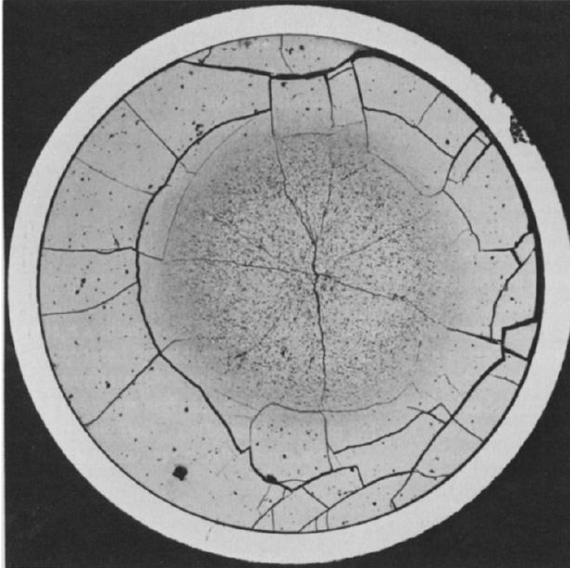
\includegraphics[width=0.7\textwidth]{Chapter345/figures/fuel}
        \end{subfigure}
        \begin{subfigure}{0.45\textwidth}
          \centering
          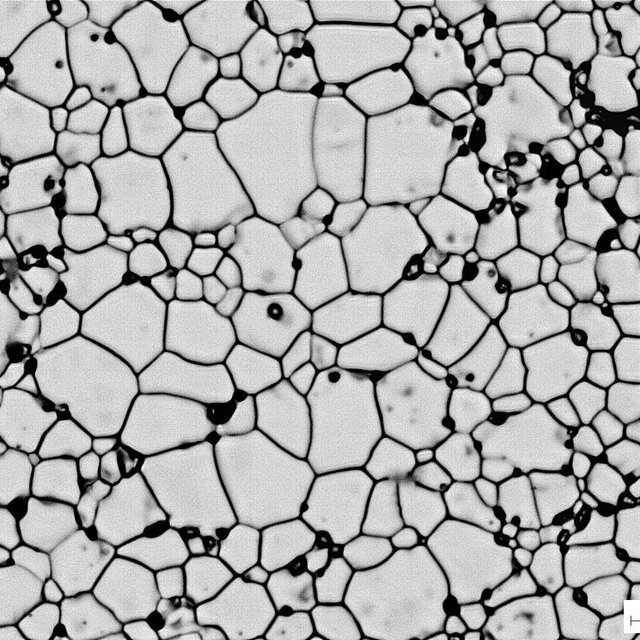
\includegraphics[width=0.7\textwidth]{Chapter345/figures/UO2_micro}
        \end{subfigure}
      \end{figure}
      
      Background:
      \begin{itemize}
        \item Fission of UO$_2$ produces a variety of fission products.
        \item Properties of UO$_2$ are strongly influenced by fracture.
        \item Gas bubbles, grains, and grain boundaries alter fracture properties.
        \item Existing 2D models over-simplifies the microstructure and results in inaccurate strength-porosity relations.
      \end{itemize}
    \end{column}
    \begin{column}{0.5\textwidth}
      Model:
      \begin{itemize}
        \item Helmholtz free energy density:
              \begin{align*}
                \psi = \psi^e + \psi^f.
              \end{align*}
        \item Strain energy density:
              \begin{align*}
                \psi^e               & = g \psi^e_\activepart + \psi^e_\inactivepart,                              \\
                \psi^e_\activepart   & = \dfrac{1}{2} \lambda \macaulay{\tr(\strain)}_+^2 + G \strain^+:\strain^+, \\
                \psi^e_\inactivepart & = \dfrac{1}{2} \lambda \macaulay{\tr(\strain)}_-^2 + G \strain^-:\strain^-, 
              \end{align*}
        \item Fracture energy density:
              \begin{align*}
                 & \psi^f = \dfrac{\Gc}{c_0 l}\left( \alpha + l^2 \grad d \cdot \grad d \right), \\
                 & \alpha = d^2, \quad g = (1-d)^2.                                              
              \end{align*}
      \end{itemize}
    \end{column}
  \end{columns}
\end{frame}

\begin{frame}
  \vspace{-1.5em}
  \begin{columns}[T]
    \begin{column}{0.6\textwidth}
      \vspace{-1em}
      \begin{figure}
        \centering
        \begin{subfigure}{0.32\textwidth}
          \centering
          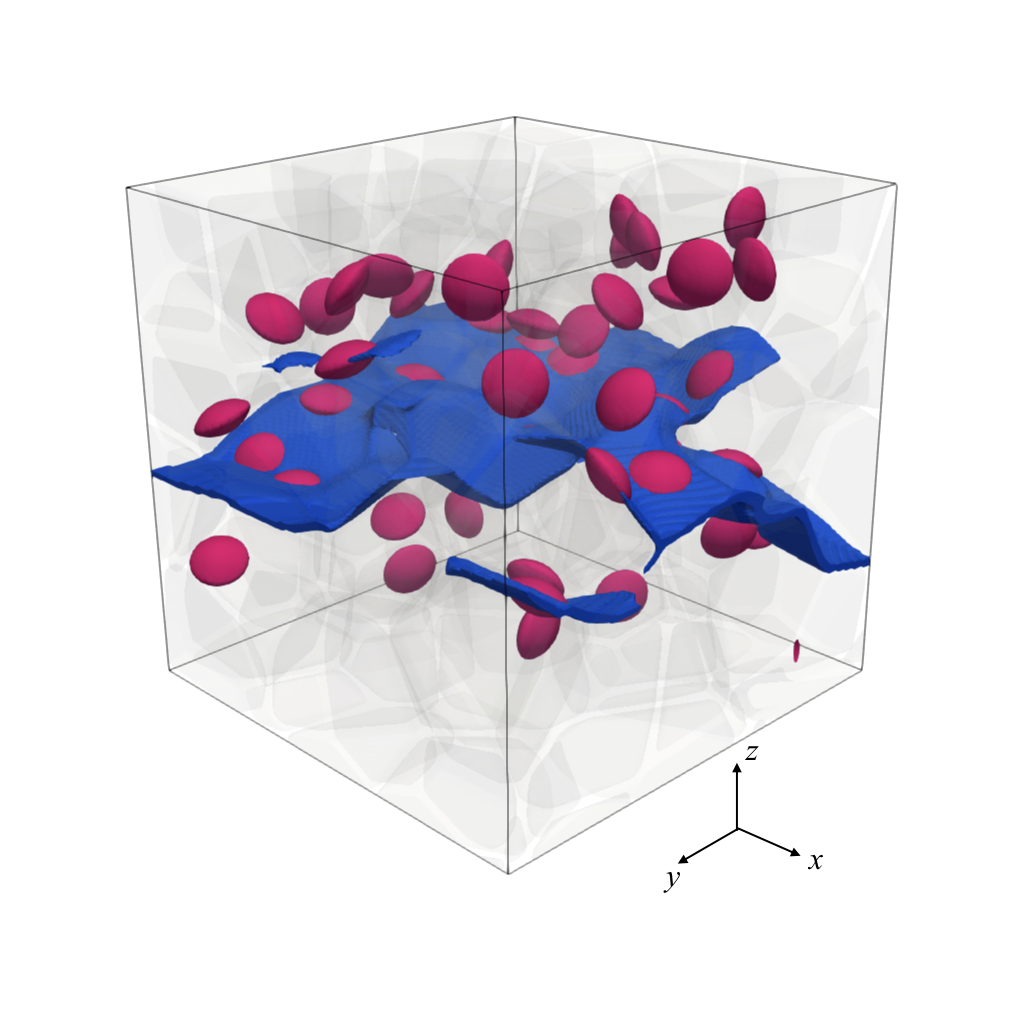
\includegraphics[width=\textwidth]{Chapter345/figures/b50_end}
        \end{subfigure}
        \begin{subfigure}{0.32\textwidth}
          \centering
          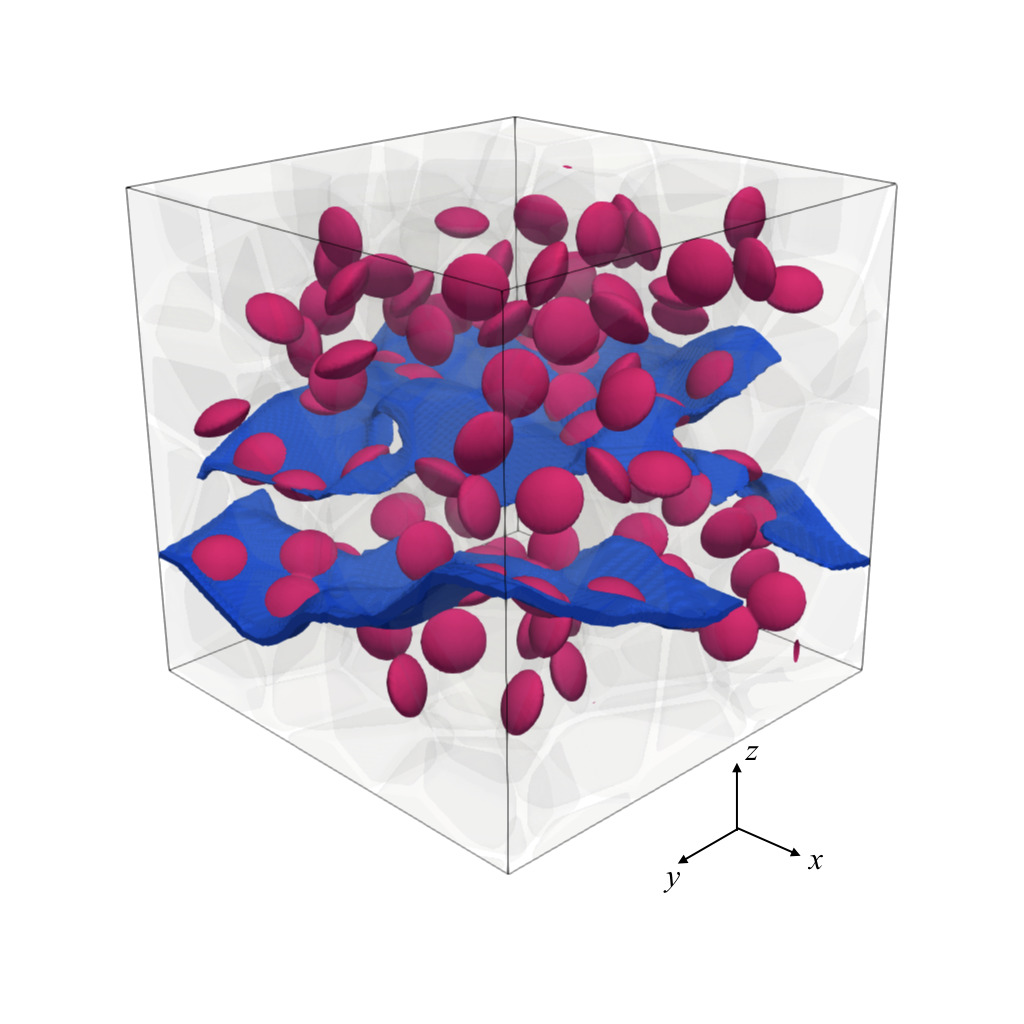
\includegraphics[width=\textwidth]{Chapter345/figures/b100_end}
        \end{subfigure}
        \begin{subfigure}{0.32\textwidth}
          \centering
          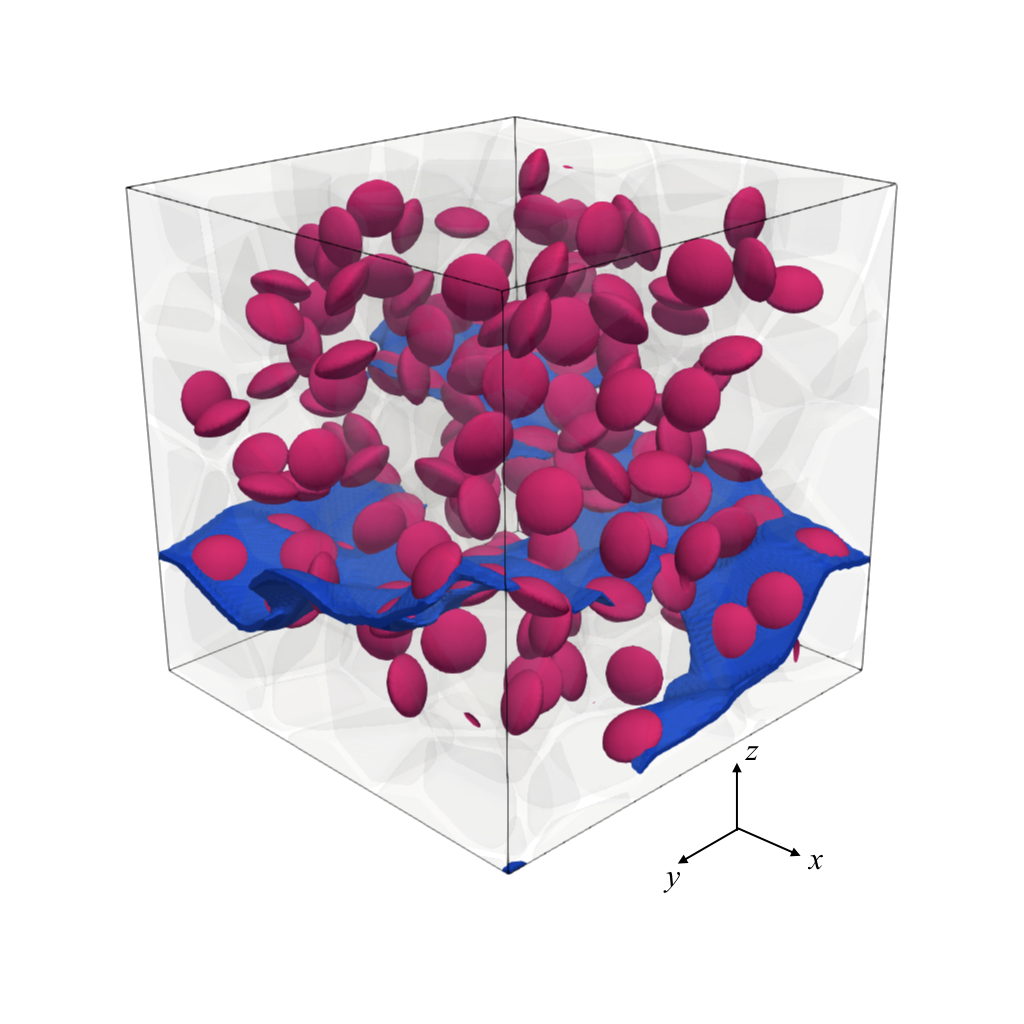
\includegraphics[width=\textwidth]{Chapter345/figures/b150_end}
        \end{subfigure}
      \end{figure}
      \begin{figure}
        \centering
        \begin{subfigure}{0.47\textwidth}
          \begin{tikzpicture}
            \begin{axis}[
                width=\textwidth,
                height=1.2\textwidth,
                xlabel=Strain,ylabel=Stress (MPa),
                xmin=0,
                xmax=0.0025,
                ymin=0,
                ymax=700,
                scaled x ticks=false,
                yticklabel style={
                    /pgf/number format/fixed,
                    /pgf/number format/precision=4
                  },
                xticklabel style={
                    /pgf/number format/fixed,
                    /pgf/number format/precision=4
                  },
                legend style={
                    at={(0.98,0.02)},
                    anchor=south east,
                    nodes={scale=0.6, transform shape},
                    draw=none,
                    fill=none
                  },
                legend cell align={left},
                every axis plot/.append style={line width=1pt,no marks,}
              ]
              \addplot +[color=black,solid] table[x expr=\thisrowno{2}/40,y=ave_stress_top] {Chapter345/data/b50_out.csv};
              \addplot +[color=black,dashed] table[x expr=\thisrowno{2}/40,y=ave_stress_top] {Chapter345/data/b100_out.csv};
              \addplot +[color=black,dotted] table[x expr=\thisrowno{2}/40,y=ave_stress_top] {Chapter345/data/b150_out.csv};
              \legend{$r = 2.02\%$,$r = 4.04\%$,$r = 6.06\%$}
            \end{axis}
          \end{tikzpicture}
        \end{subfigure}
        \begin{subfigure}{0.47\textwidth}
          \begin{tikzpicture}
            \begin{axis}[
                width=\textwidth,
                height=1.2\textwidth,
                xlabel=Porosity (\%),ylabel=$\sigma_c^*$,
                xmin=0,
                xmax=10,
                ymin=0,
                ymax=1.2,
                legend style={
                    at={(0.05,0.05)},
                    anchor=south west,
                    nodes={scale=0.6, transform shape},
                    draw=none,
                    fill=none
                  },
                legend cell align={left},
                every axis plot/.append style={line width=1pt}
              ]
              % plot the confidence interval band
              \addplot [name path=upper,draw=none,domain=0:10,forget plot] {727/697.8*exp(-0.02925*x)};
              \addplot [name path=lower,draw=none,domain=0:10,forget plot] {668.5/697.8*exp(-0.04959*x)};
              \tikzfillbetween[of=upper and lower]{pattern=north west lines};
              % experiment
              \addplot +[mark=none,color=black,solid,domain=0:10] {exp(-0.057*x)};
              % 3D
              \addplot +[mark=none,color=black,dashed,domain=0:10] {exp(-0.03942*x)};
              % 2D
              \addplot +[mark=none,color=black,dotted,domain=0:10] {exp(-0.14*x)};
              \legend{Experiment,3D simulation,2D simulation}
            \end{axis}
          \end{tikzpicture}
        \end{subfigure}
      \end{figure}
    \end{column}
    \begin{column}{0.4\textwidth}
      \begin{itemize}
        \item A set of random close-packing voronoi structures are realized by maximal Poisson-disk sampling.
        \item The microstructure is generated using a phase-field grain growth model \cite{Moelans2008}.
        \item Grain boundaries have an arbitrarily high fracture toughness to facilitate intergranular fracture.
        \item Numerical studies are performed to investigate the effects of bubble geometry, loading conditions, and porosity on the critical fracture strength.
        \item Results of 15 realizations of 3 porosity levels are fitted using the relation suggested by experiments \cite{oguma_1982}:
              \begin{align*}
                \dfrac{\sigma_c}{\sigma_0} = \exp(-a r).
              \end{align*}
      \end{itemize}
    \end{column}
  \end{columns}
\end{frame}

\begin{frame}
  \vspace{-1.5em}
  \begin{columns}[T]
    \begin{column}{0.5\textwidth}
      \begin{figure}
        \centering
        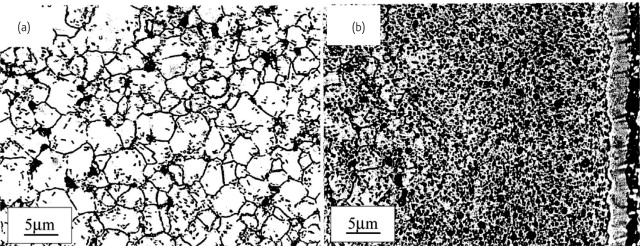
\includegraphics[width=0.8\textwidth]{Chapter345/figures/HBS}
      \end{figure}
      
      Background:
      \begin{itemize}
        \item Utilities are seeking to increase the allowable burnup limit for UO$_2$ fuel.
        \item The risk of fragmentation during a loss-of-coolant accident (LOCA) is a major limitation.
        \item Over-pressurization of fission gas bubbles results in fine fragmentation of high burnup structures.
        \item A model for predicting the onset of fragmentation is essential.
      \end{itemize}
    \end{column}
    \begin{column}{0.5\textwidth}
      External pressure power:
      \begin{align*}
        \mathcal{P}^\text{ext} = - \int\limits_{\body_0} \bar{p} \grad d \cdot \defrate I_{,d} \diff{V}.
      \end{align*}
      \begin{figure}
        \centering
        \begin{subfigure}[b]{0.95\textwidth}
          \centering
          \begin{tikzpicture}
            \begin{axis}[
                colormap/jet,
                cycle list={[of colormap,samples of colormap=5]},
                width=\textwidth,
                height=0.5\textwidth,
                xmin=0,
                xmax=0.1,
                ymin=0,
                xlabel=$w$ (\SI{}{\milli\meter}),
                ylabel=$t$ (\SI{}{\newton}),
                scaled x ticks=false,
                yticklabel style={
                    /pgf/number format/fixed,
                    /pgf/number format/precision=2
                  },
                xticklabel style={
                    /pgf/number format/fixed,
                    /pgf/number format/precision=2
                  },
                legend style={
                    at={(0.97,0.97)},
                    anchor=north east,
                    nodes={scale=0.6, transform shape},
                    fill=none,
                    draw=none,
                    text opacity=1,
                    cells={align=left}
                  },
                legend cell align={left},
                every axis plot/.append style={no marks}
              ]
              \addplot table[x=separation,y expr=-\thisrowno{1},col sep=comma]{Chapter345/data/force_disp_p_0_r_5.csv};
              \addplot table[x=separation,y expr=-\thisrowno{1},col sep=comma]{Chapter345/data/force_disp_p_0.25_r_5.csv};
              \addplot table[x=separation,y expr=-\thisrowno{1},col sep=comma]{Chapter345/data/force_disp_p_0.5_r_5.csv};
              \addplot table[x=separation,y expr=-\thisrowno{1},col sep=comma]{Chapter345/data/force_disp_p_0.75_r_5.csv};
              \addplot table[x=separation,y expr=-\thisrowno{1},col sep=comma]{Chapter345/data/force_disp_p_1_r_5.csv};
              \legend{$p=\SI{0}{\mega\pascal}$,$p=\SI{0.25}{\mega\pascal}$,$p=\SI{0.5}{\mega\pascal}$,$p=\SI{0.75}{\mega\pascal}$,$p=\SI{1}{\mega\pascal}$}
            \end{axis}
          \end{tikzpicture}
        \end{subfigure}
        
        \begin{subfigure}[b]{0.95\textwidth}
          \centering
          \begin{tikzpicture}
            \begin{axis}[
                colormap/jet,
                cycle list={[of colormap,samples of colormap=5]},
                width=\textwidth,
                height=0.5\textwidth,
                xmin=0,
                xmax=0.1,
                ymin=0,
                xlabel=$w$ (\SI{}{\milli\meter}),
                ylabel=$t$ (\SI{}{\newton}),
                scaled x ticks=false,
                yticklabel style={
                    /pgf/number format/fixed,
                    /pgf/number format/precision=2
                  },
                xticklabel style={
                    /pgf/number format/fixed,
                    /pgf/number format/precision=2
                  },
                legend style={
                    at={(0.97,0.97)},
                    anchor=north east,
                    nodes={scale=0.6, transform shape},
                    fill=none,
                    draw=none,
                    text opacity=1,
                    cells={align=left}
                  },
                legend cell align={left},
                every axis plot/.append style={no marks}
              ]
              \addplot table[x=separation,y expr=-\thisrowno{1},col sep=comma]{Chapter345/data/force_disp_p_0.25_r_5_l_2.csv};
              \addplot table[x=separation,y expr=-\thisrowno{1},col sep=comma]{Chapter345/data/force_disp_p_0.25_r_5_l_5.csv};
              \addplot table[x=separation,y expr=-\thisrowno{1},col sep=comma]{Chapter345/data/force_disp_p_0.25_r_5_l_10.csv};
              \addplot table[x=separation,y expr=-\thisrowno{1},col sep=comma]{Chapter345/data/force_disp_p_0.25_r_5_l_20.csv};
              \addplot table[x=separation,y expr=-\thisrowno{1},col sep=comma]{Chapter345/data/force_disp_p_0.25_r_5_l_50.csv};
              \legend{$l=\SI{2}{\milli\meter}$,$l=\SI{5}{\milli\meter}$,$l=\SI{10}{\milli\meter}$,$l=\SI{20}{\milli\meter}$,$l=\SI{50}{\milli\meter}$}
            \end{axis}
          \end{tikzpicture}
        \end{subfigure}
      \end{figure}
    \end{column}
  \end{columns}
\end{frame}

\begin{frame}
  \vspace{-1.5em}
  \begin{columns}[T]
    \begin{column}{0.2\textwidth}
      \vspace{-1em}
      \begin{figure}
        \centering
        \begin{subfigure}{0.94\linewidth}
          \centering
          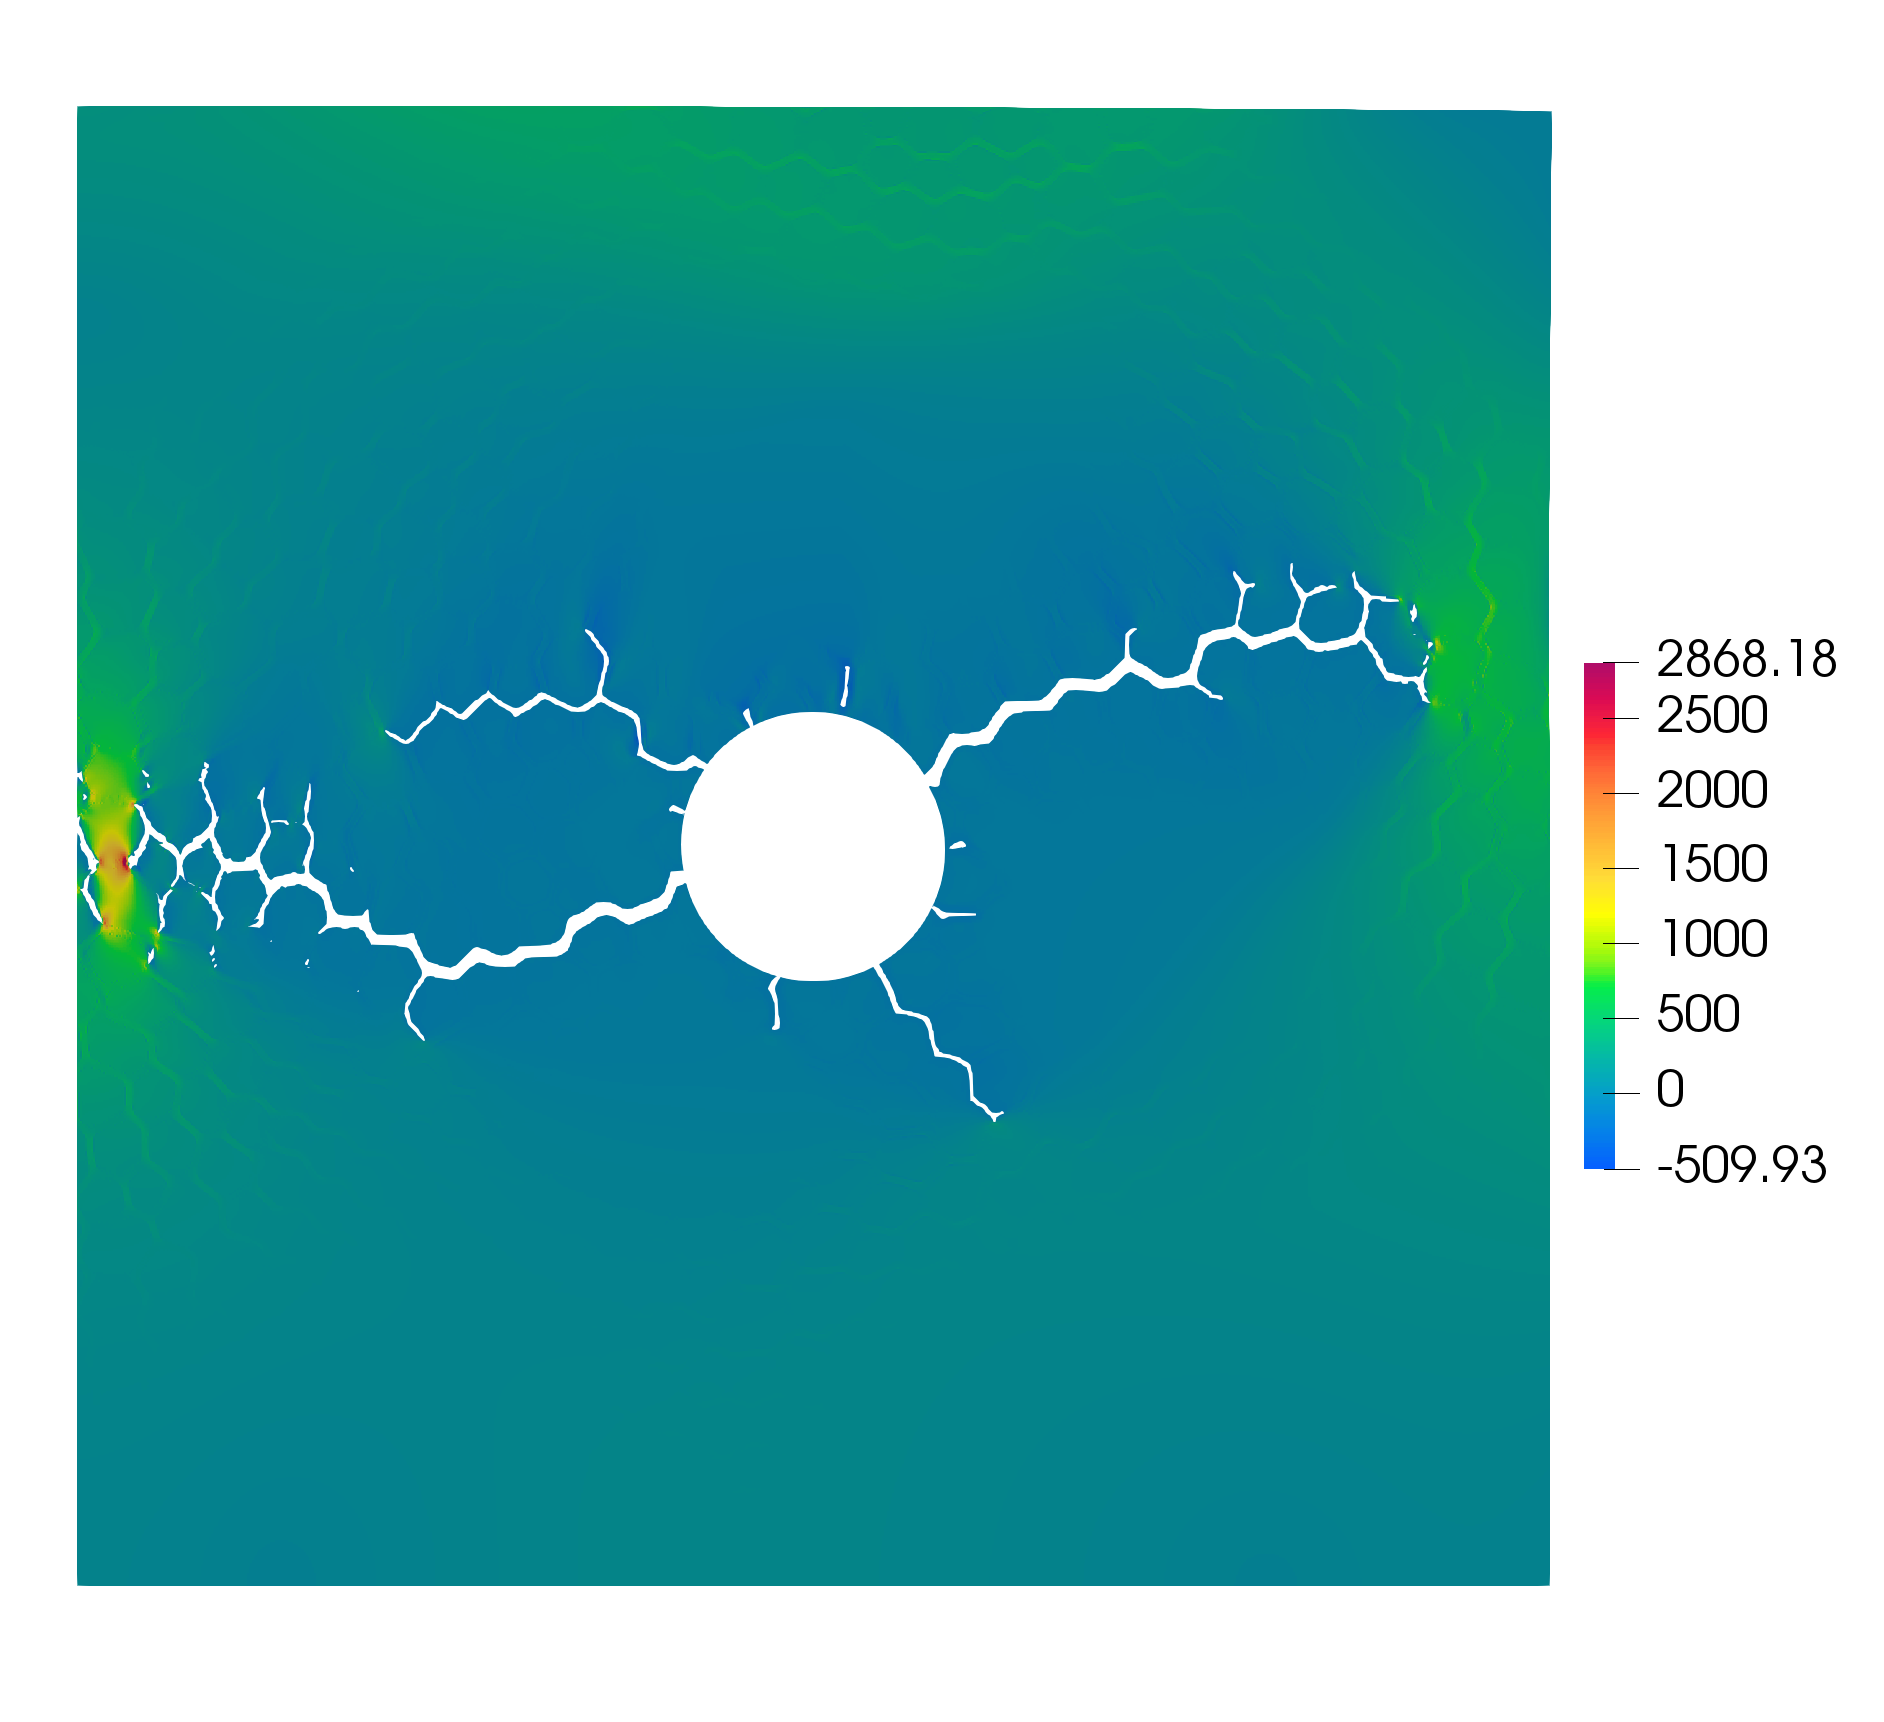
\includegraphics[width=0.9\linewidth]{Chapter345/figures/r25_ext0_stress}
        \end{subfigure}
        \begin{subfigure}{0.94\linewidth}
          \centering
          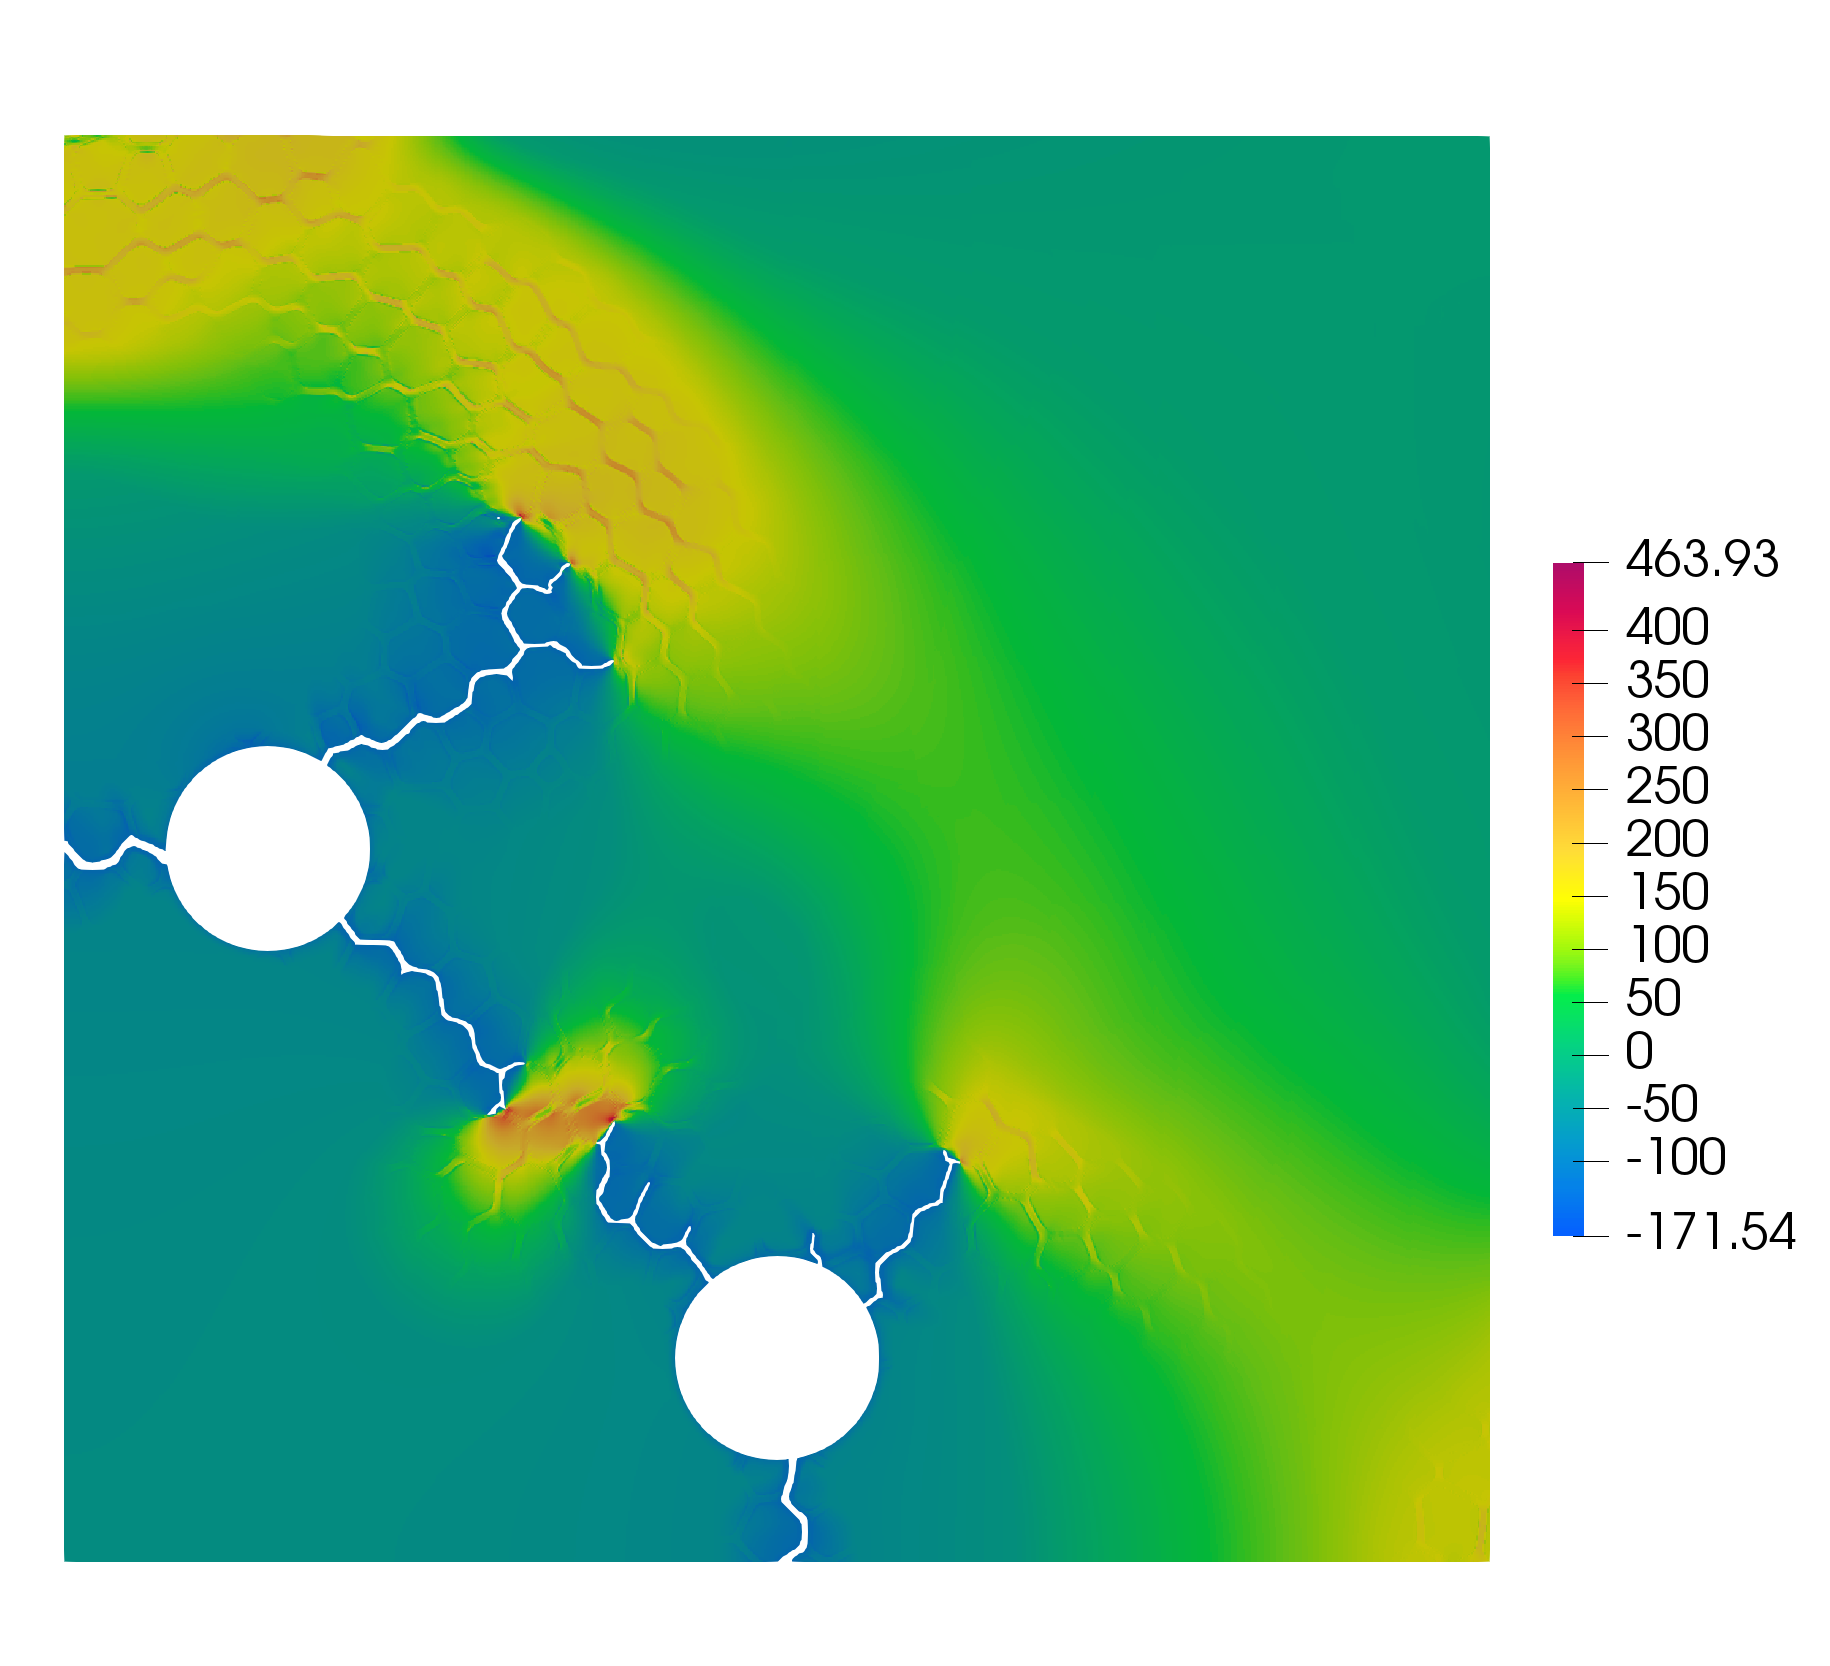
\includegraphics[width=0.9\linewidth]{Chapter345/figures/two_bubbles_stress}
        \end{subfigure}
        \begin{subfigure}{0.94\linewidth}
          \centering
          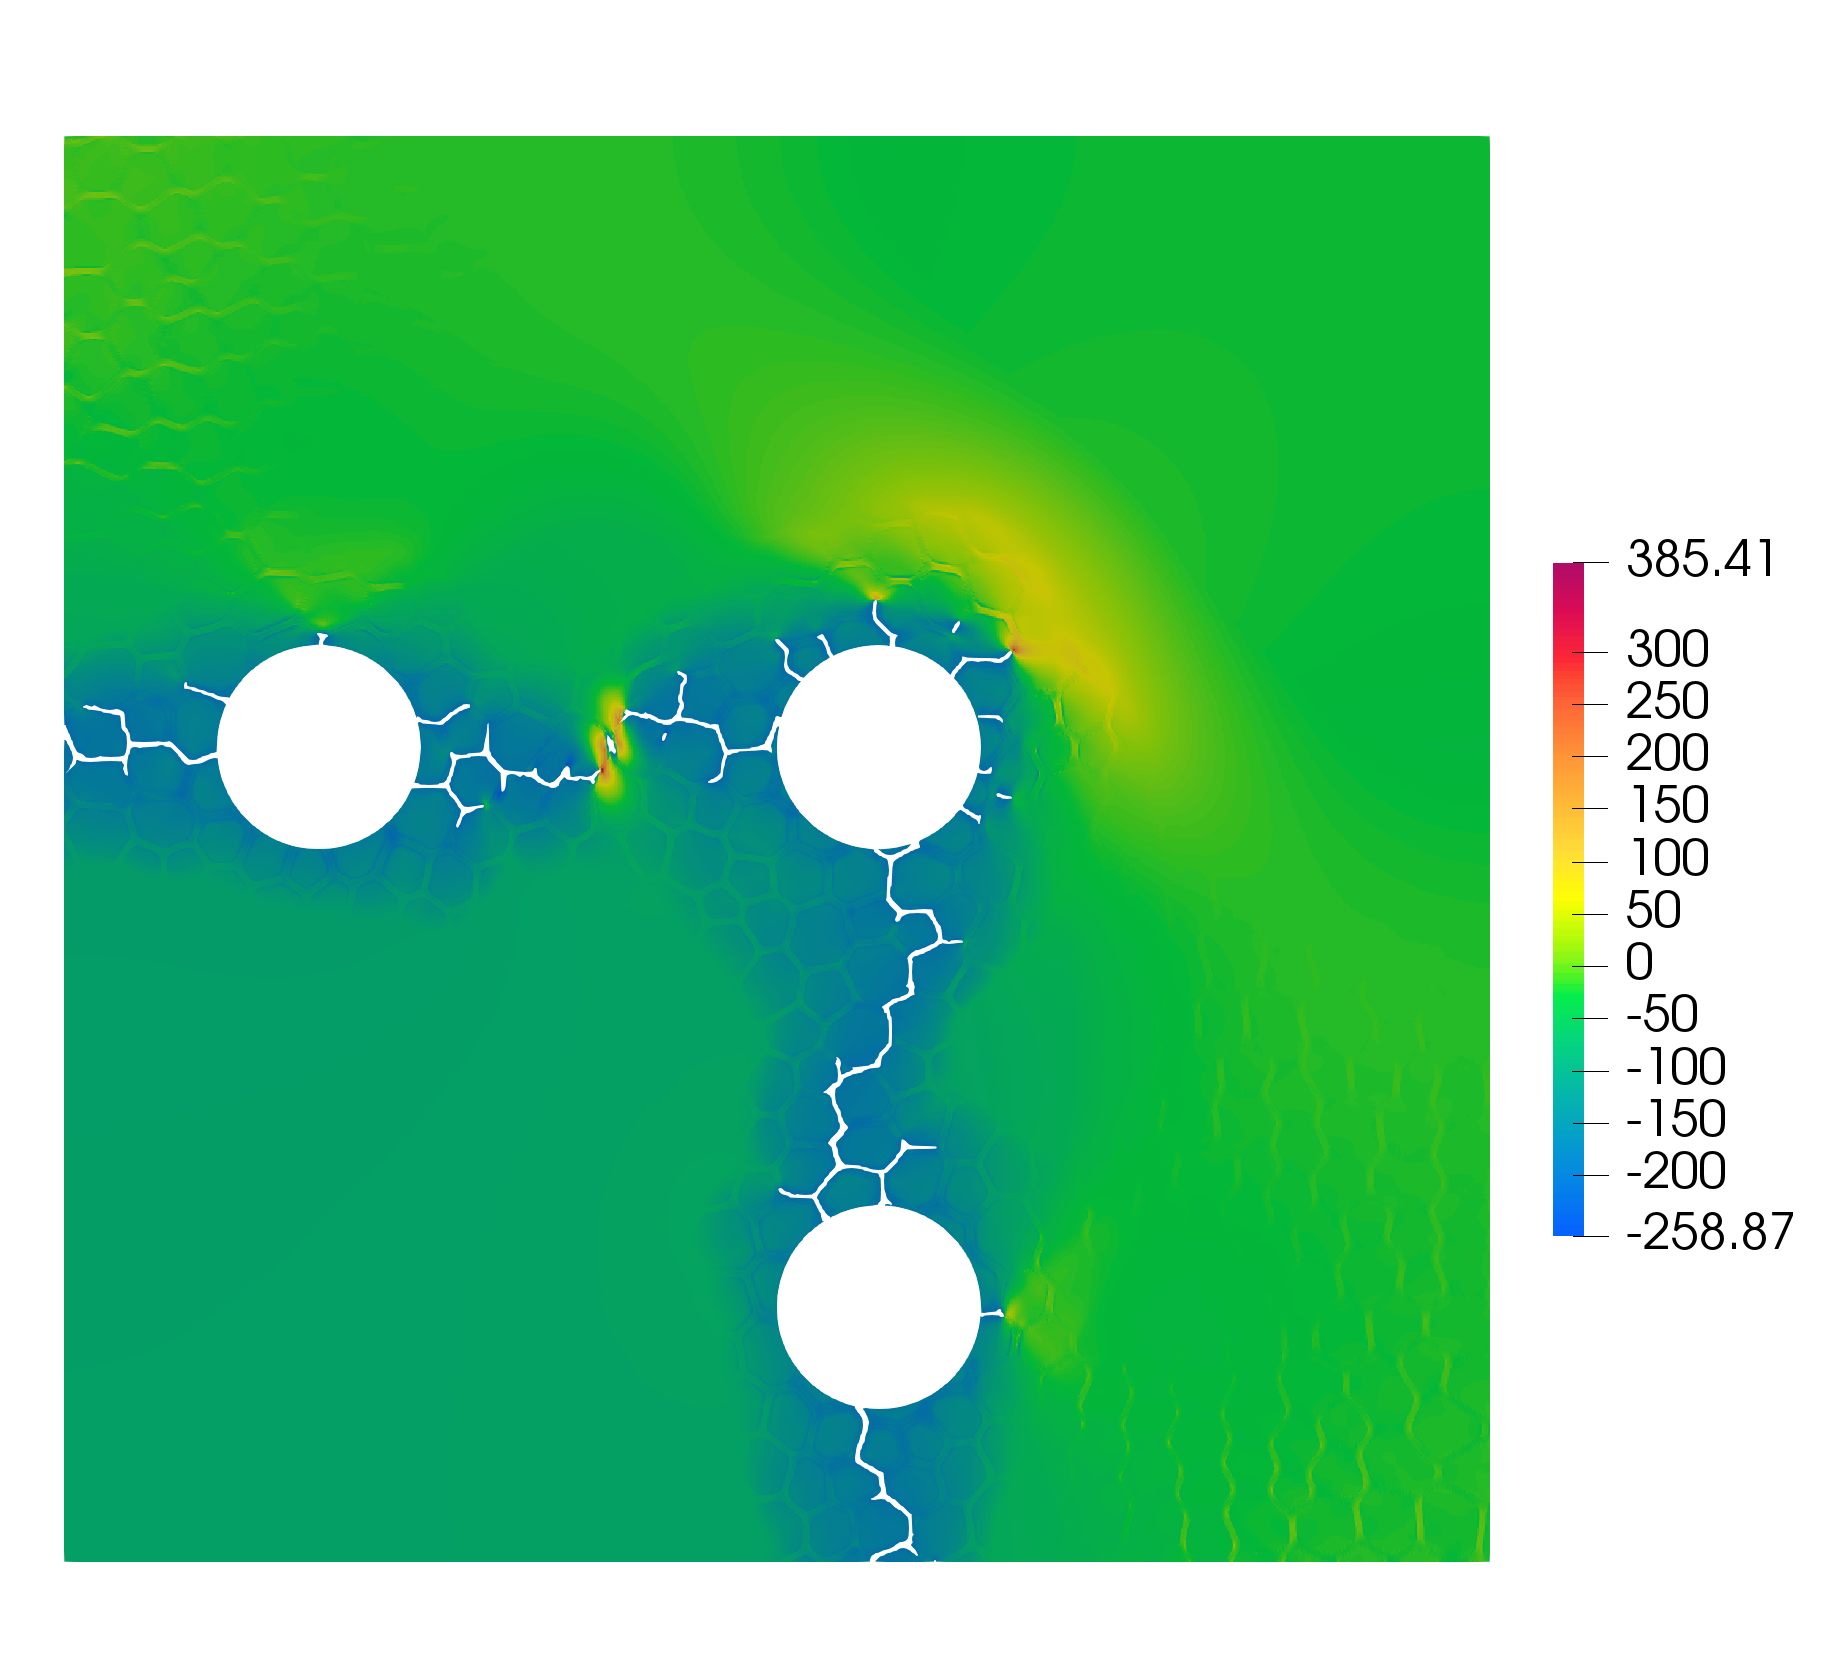
\includegraphics[width=0.9\linewidth]{Chapter345/figures/three_bubbles_stress}
        \end{subfigure}
      \end{figure}
    \end{column}
    \begin{column}{0.4\textwidth}
      \vspace{-1em}
      \begin{figure}
        \centering
        \begin{subfigure}[t]{0.47\linewidth}
          \centering
          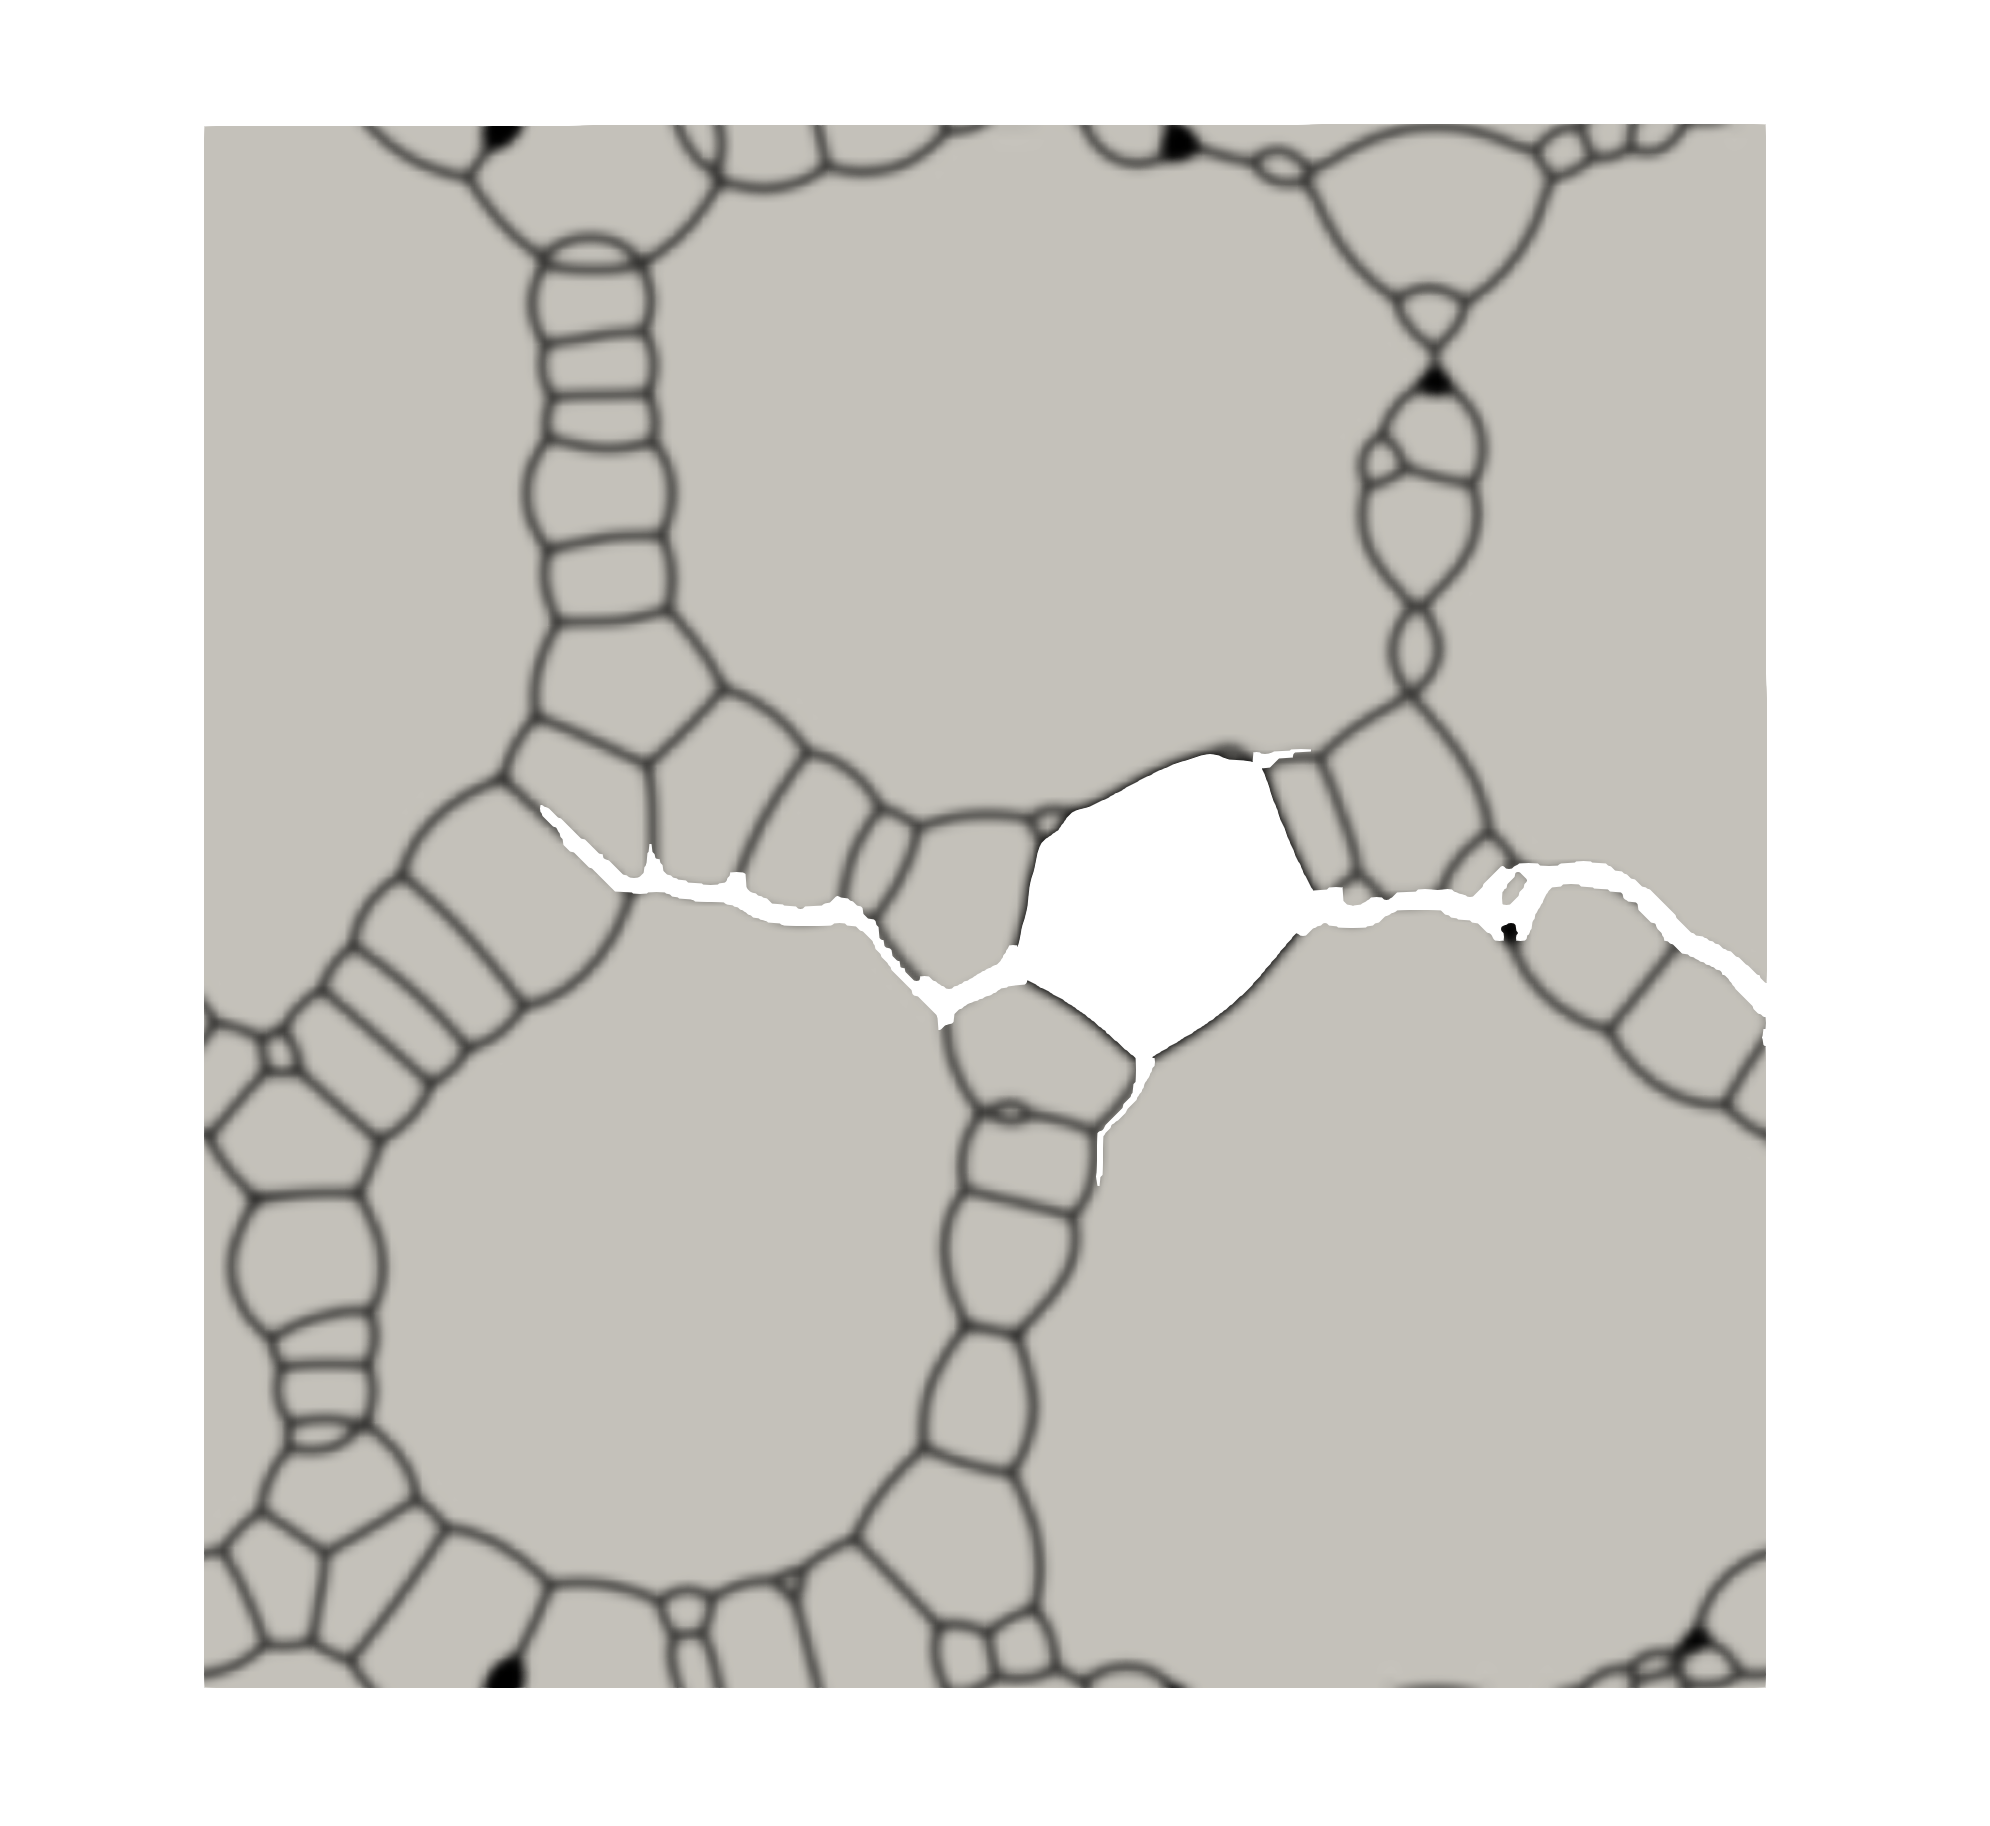
\includegraphics[width=0.9\linewidth]{Chapter345/figures/partial_hbs_1}
        \end{subfigure}
        \begin{subfigure}[t]{0.47\linewidth}
          \centering
          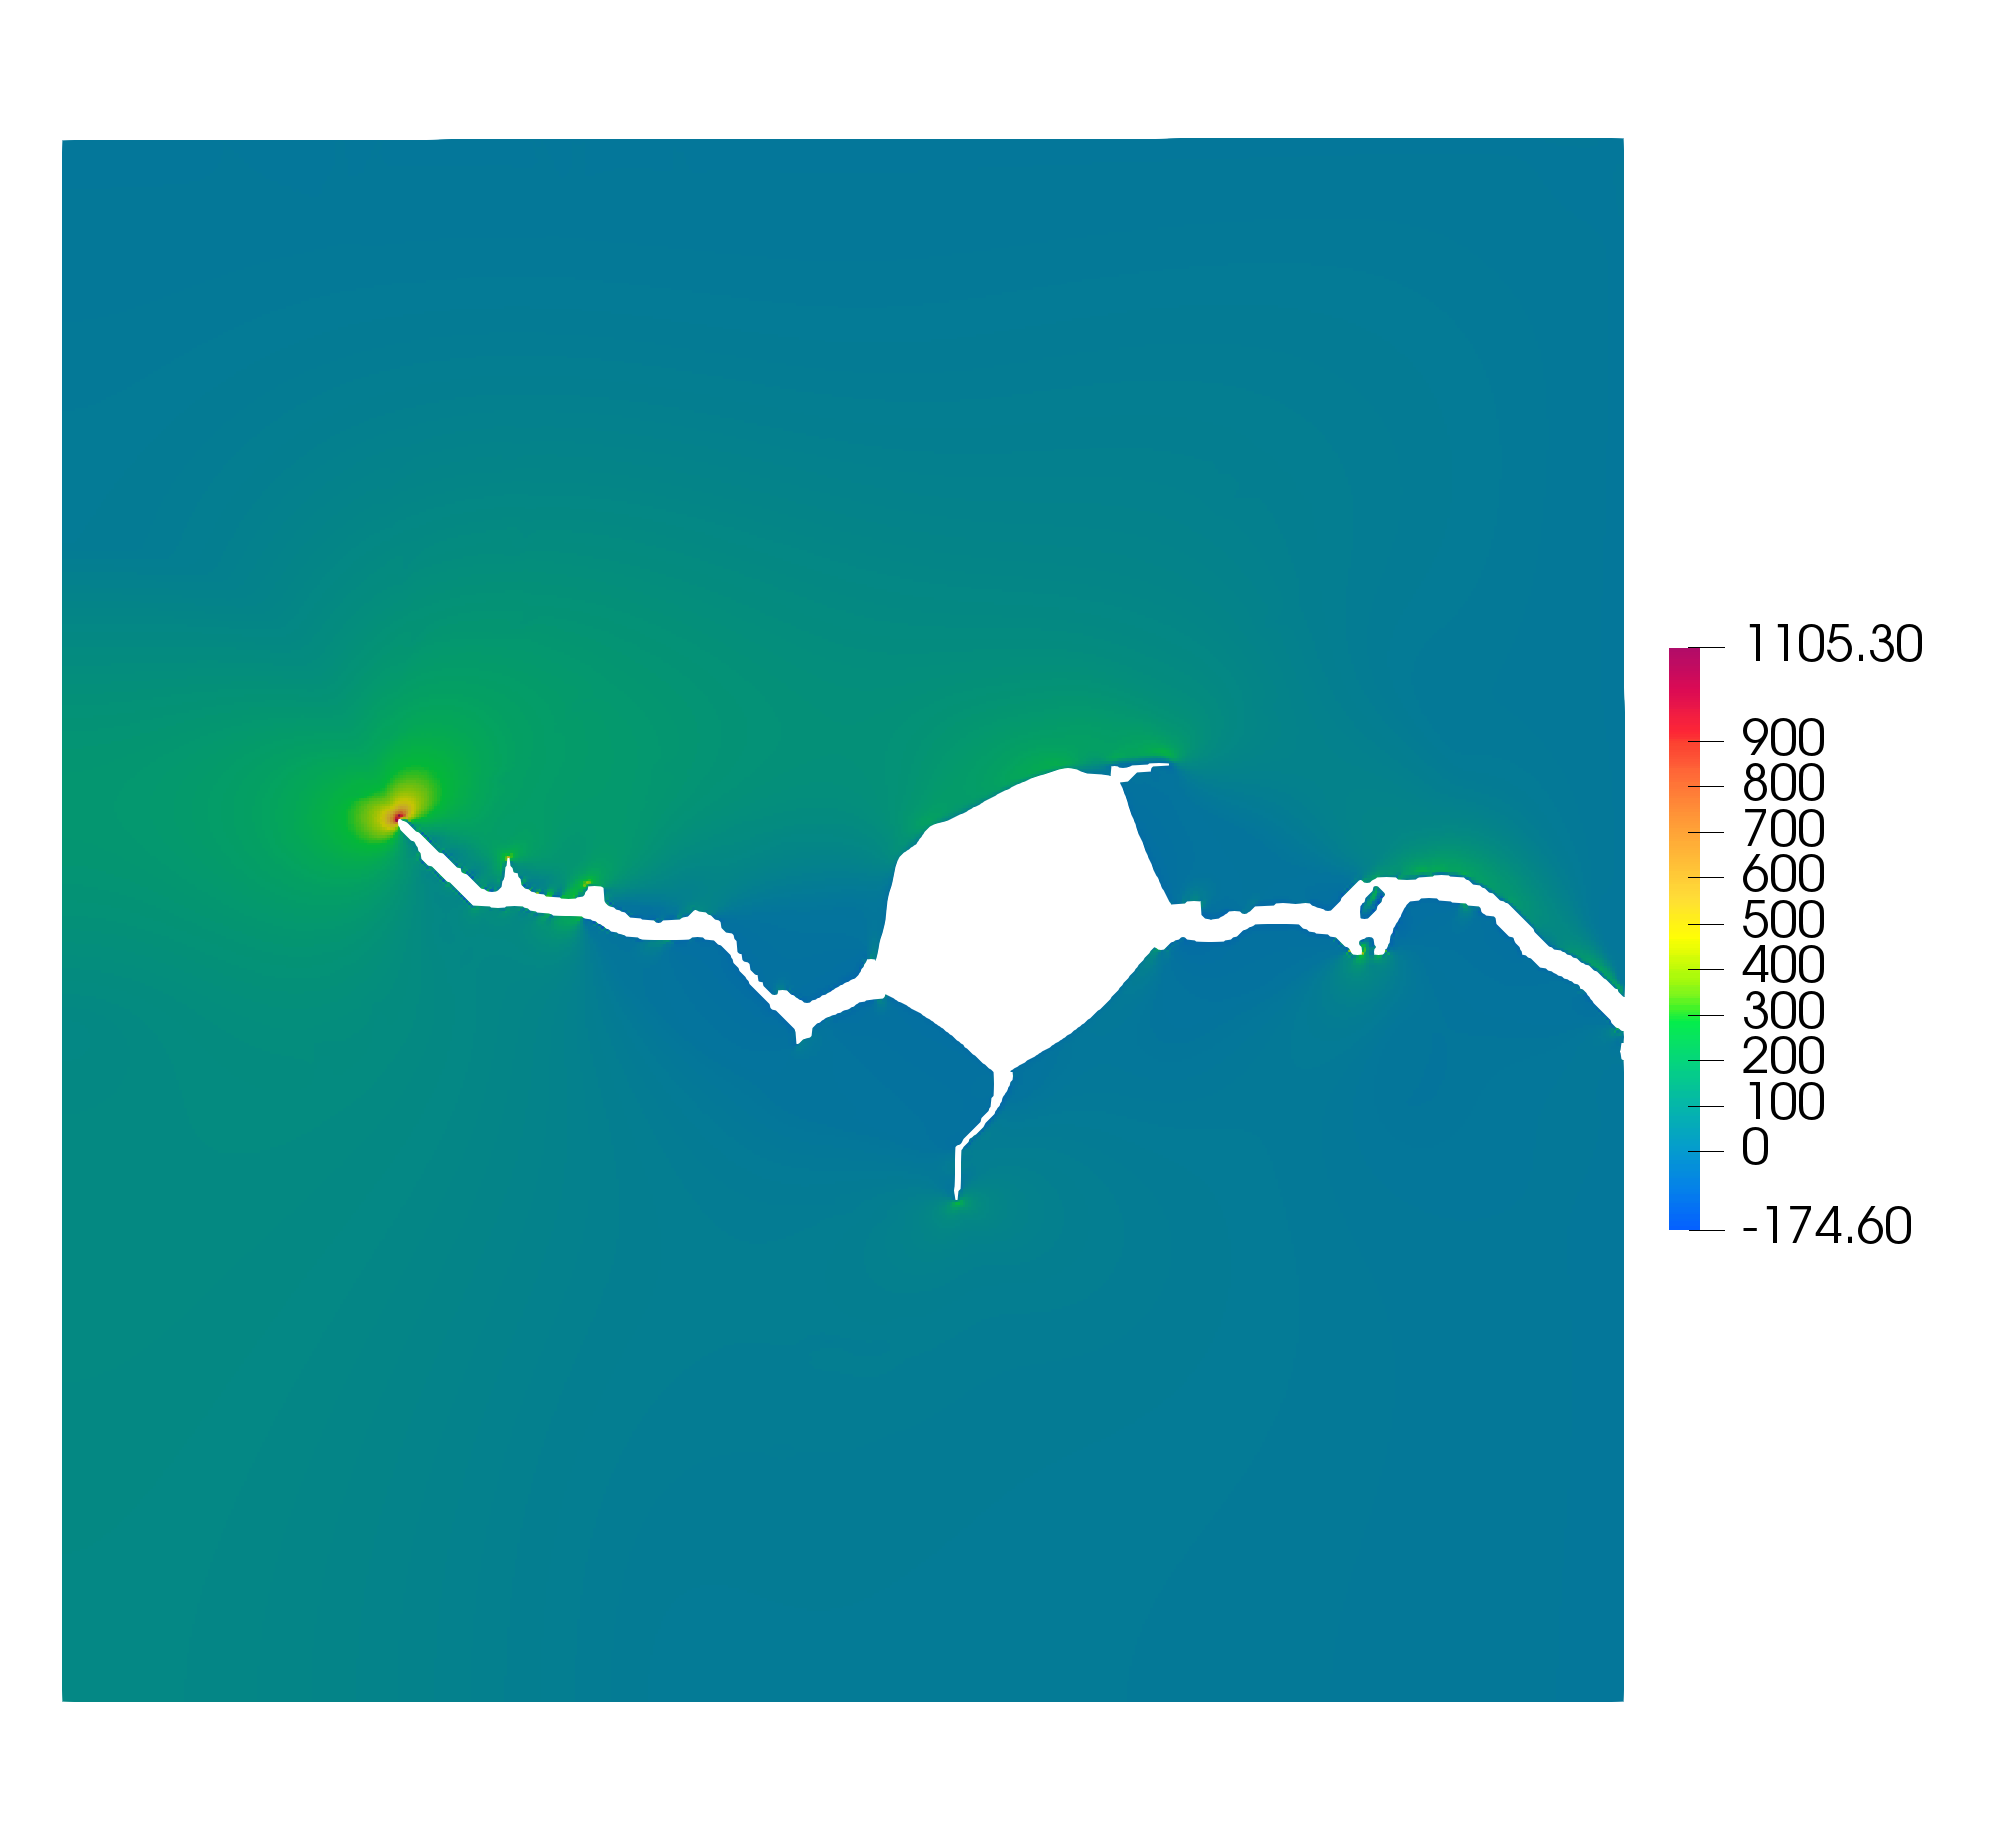
\includegraphics[width=0.9\linewidth]{Chapter345/figures/partial_hbs_1_stress}
        \end{subfigure}
        
        \begin{subfigure}[t]{0.47\linewidth}
          \centering
          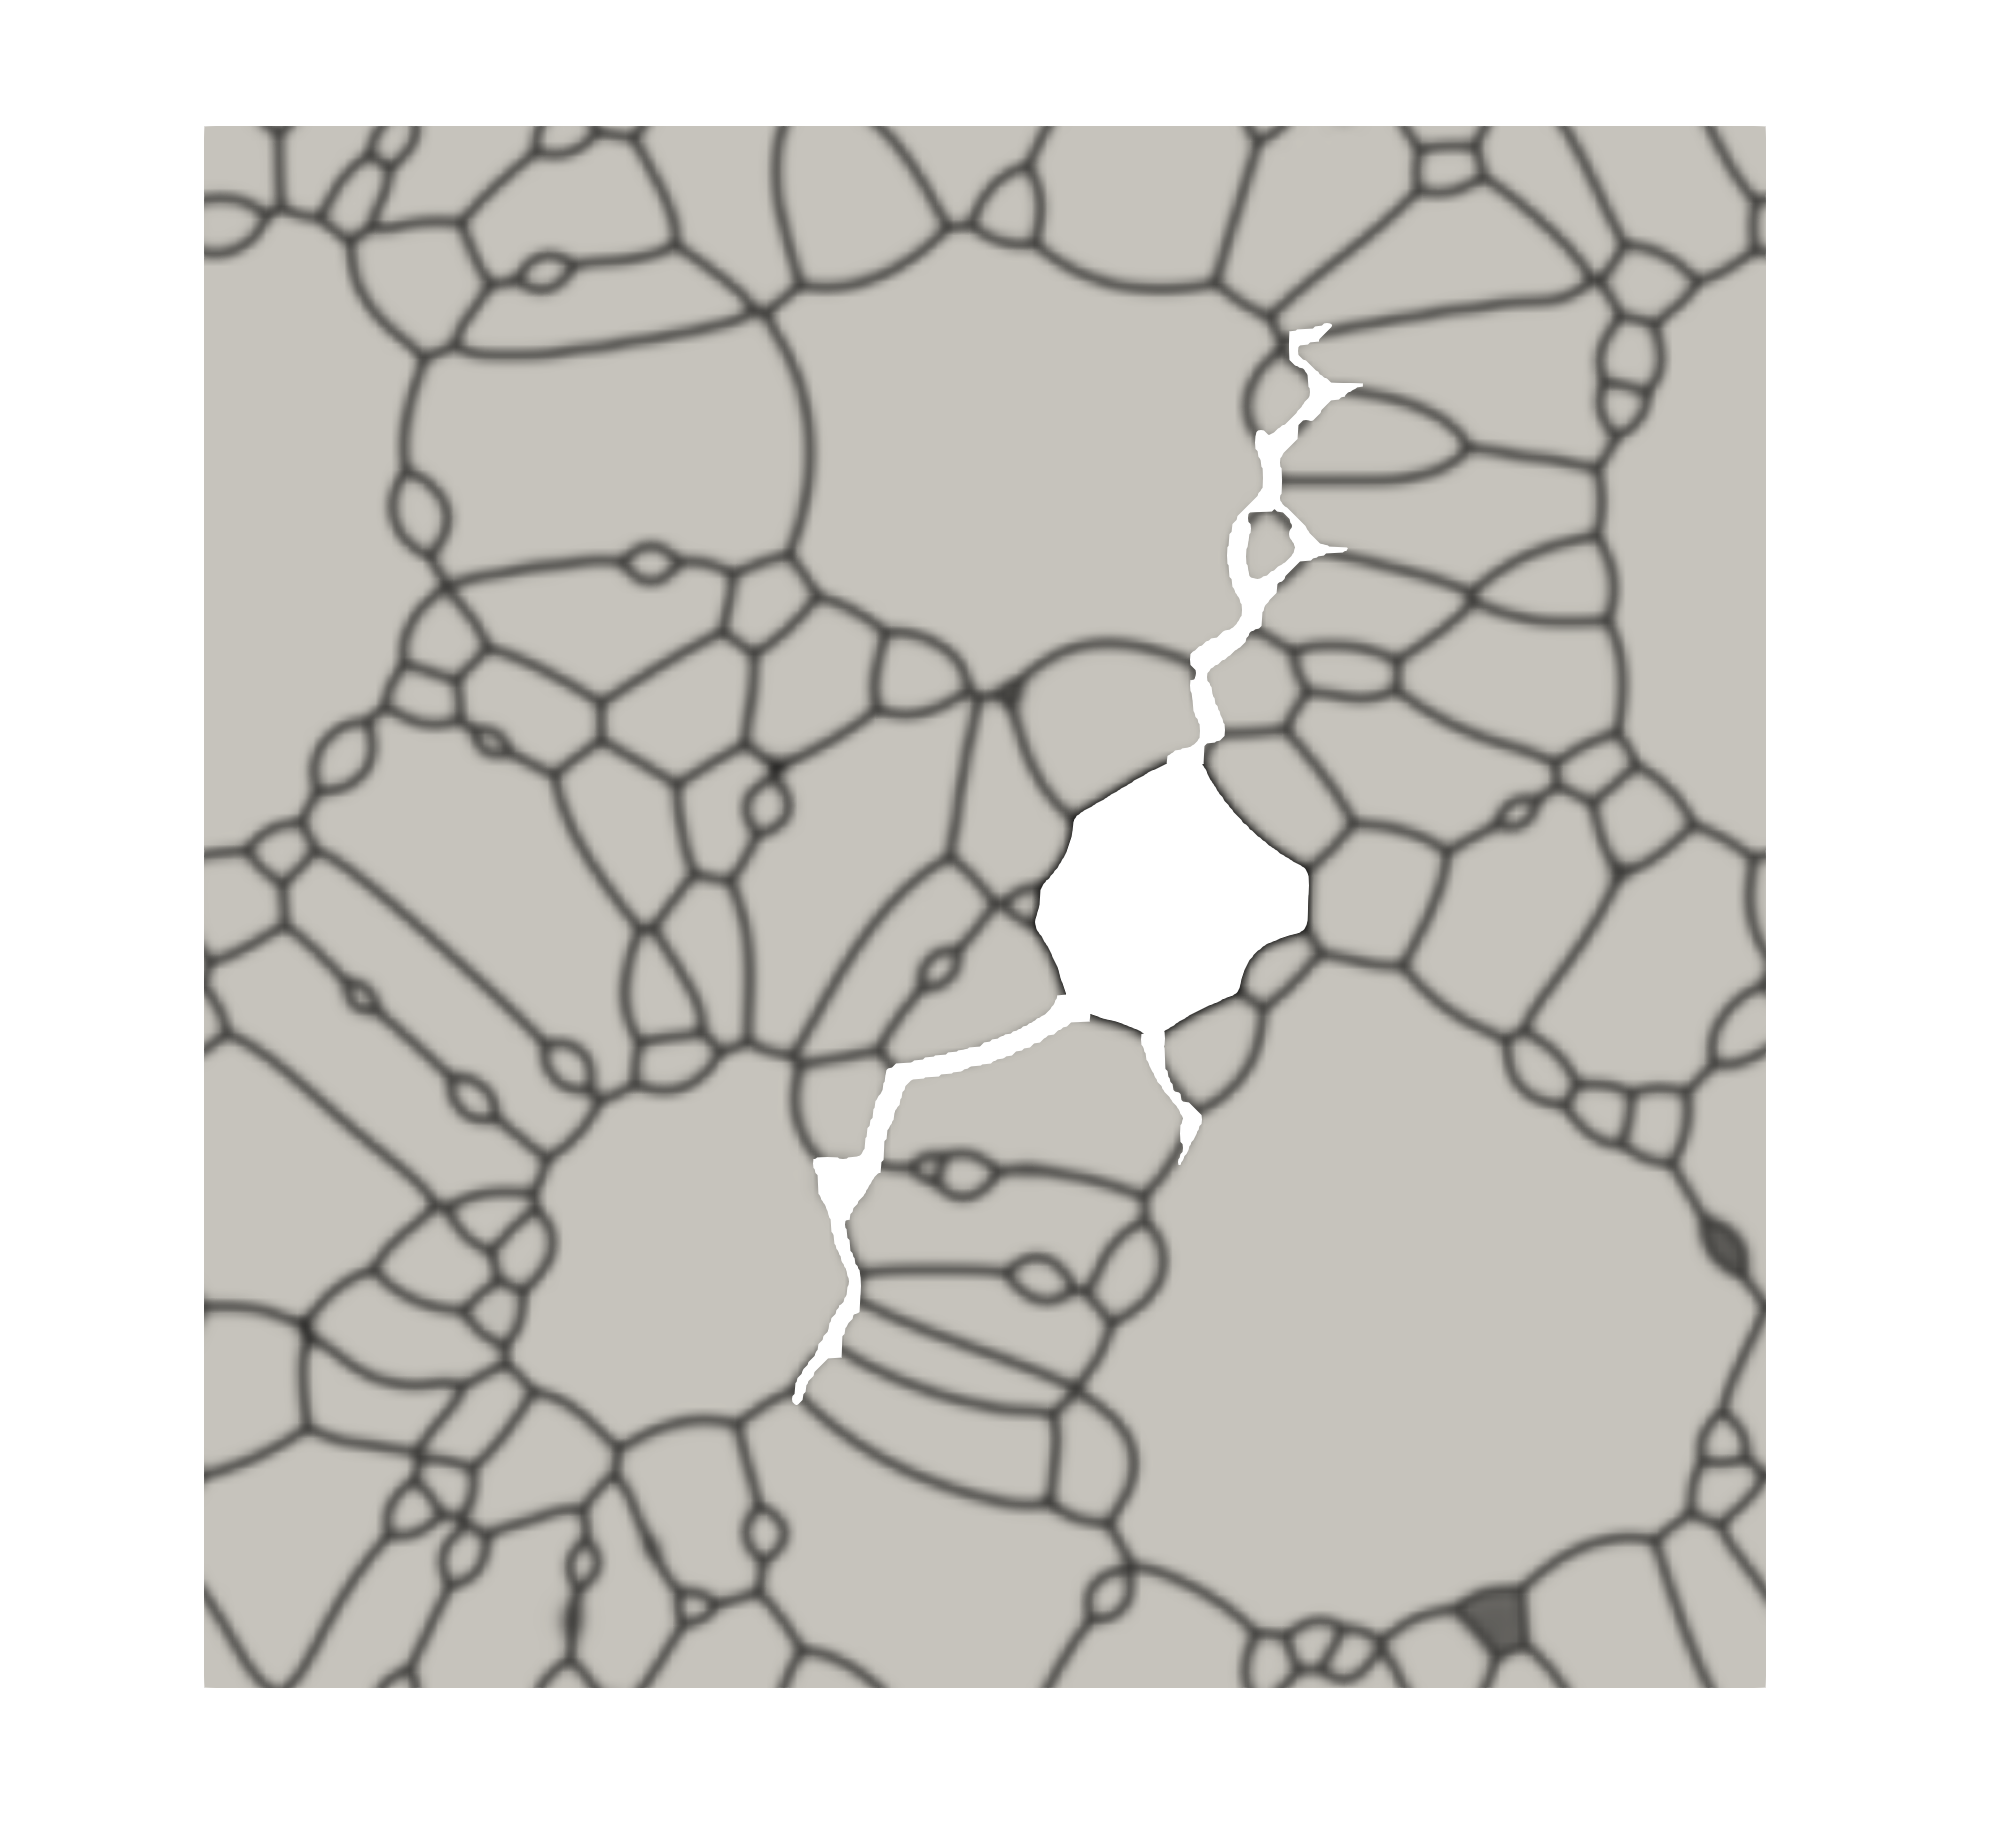
\includegraphics[width=0.9\linewidth]{Chapter345/figures/partial_hbs_2}
        \end{subfigure}
        \begin{subfigure}[t]{0.47\linewidth}
          \centering
          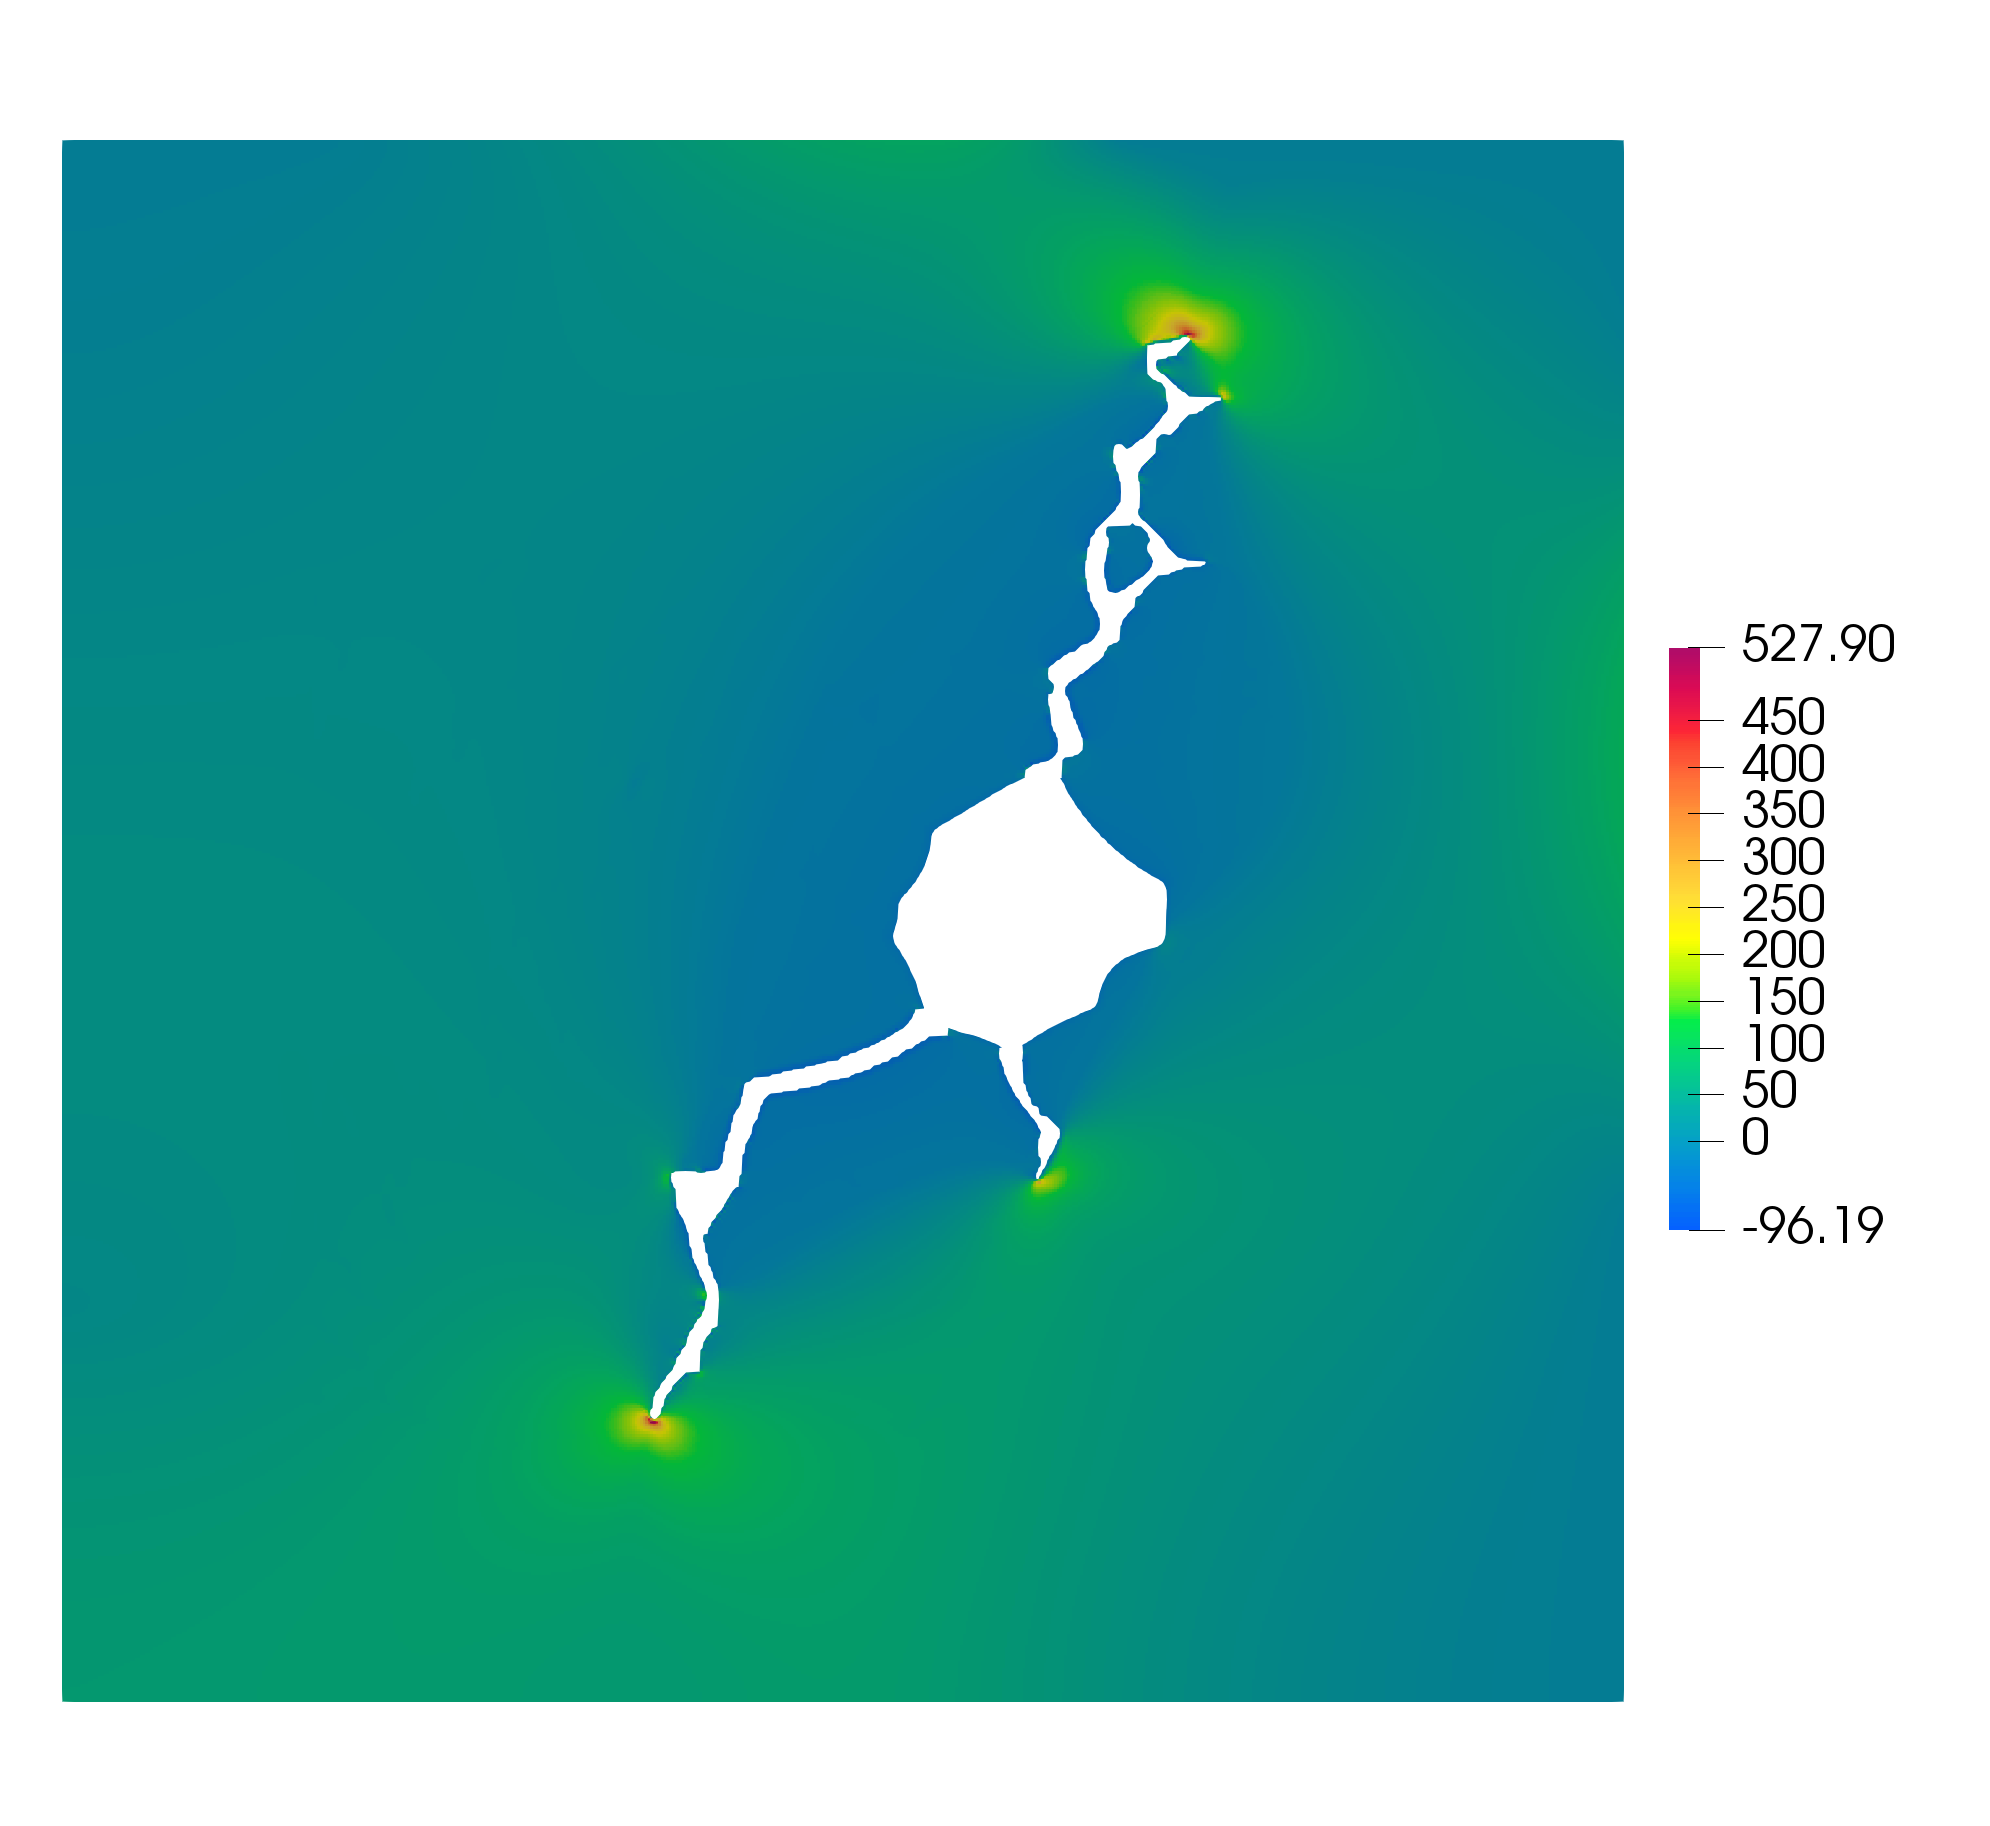
\includegraphics[width=0.9\linewidth]{Chapter345/figures/partial_hbs_2_stress}
        \end{subfigure}
        
        \begin{subfigure}[t]{0.47\linewidth}
          \centering
          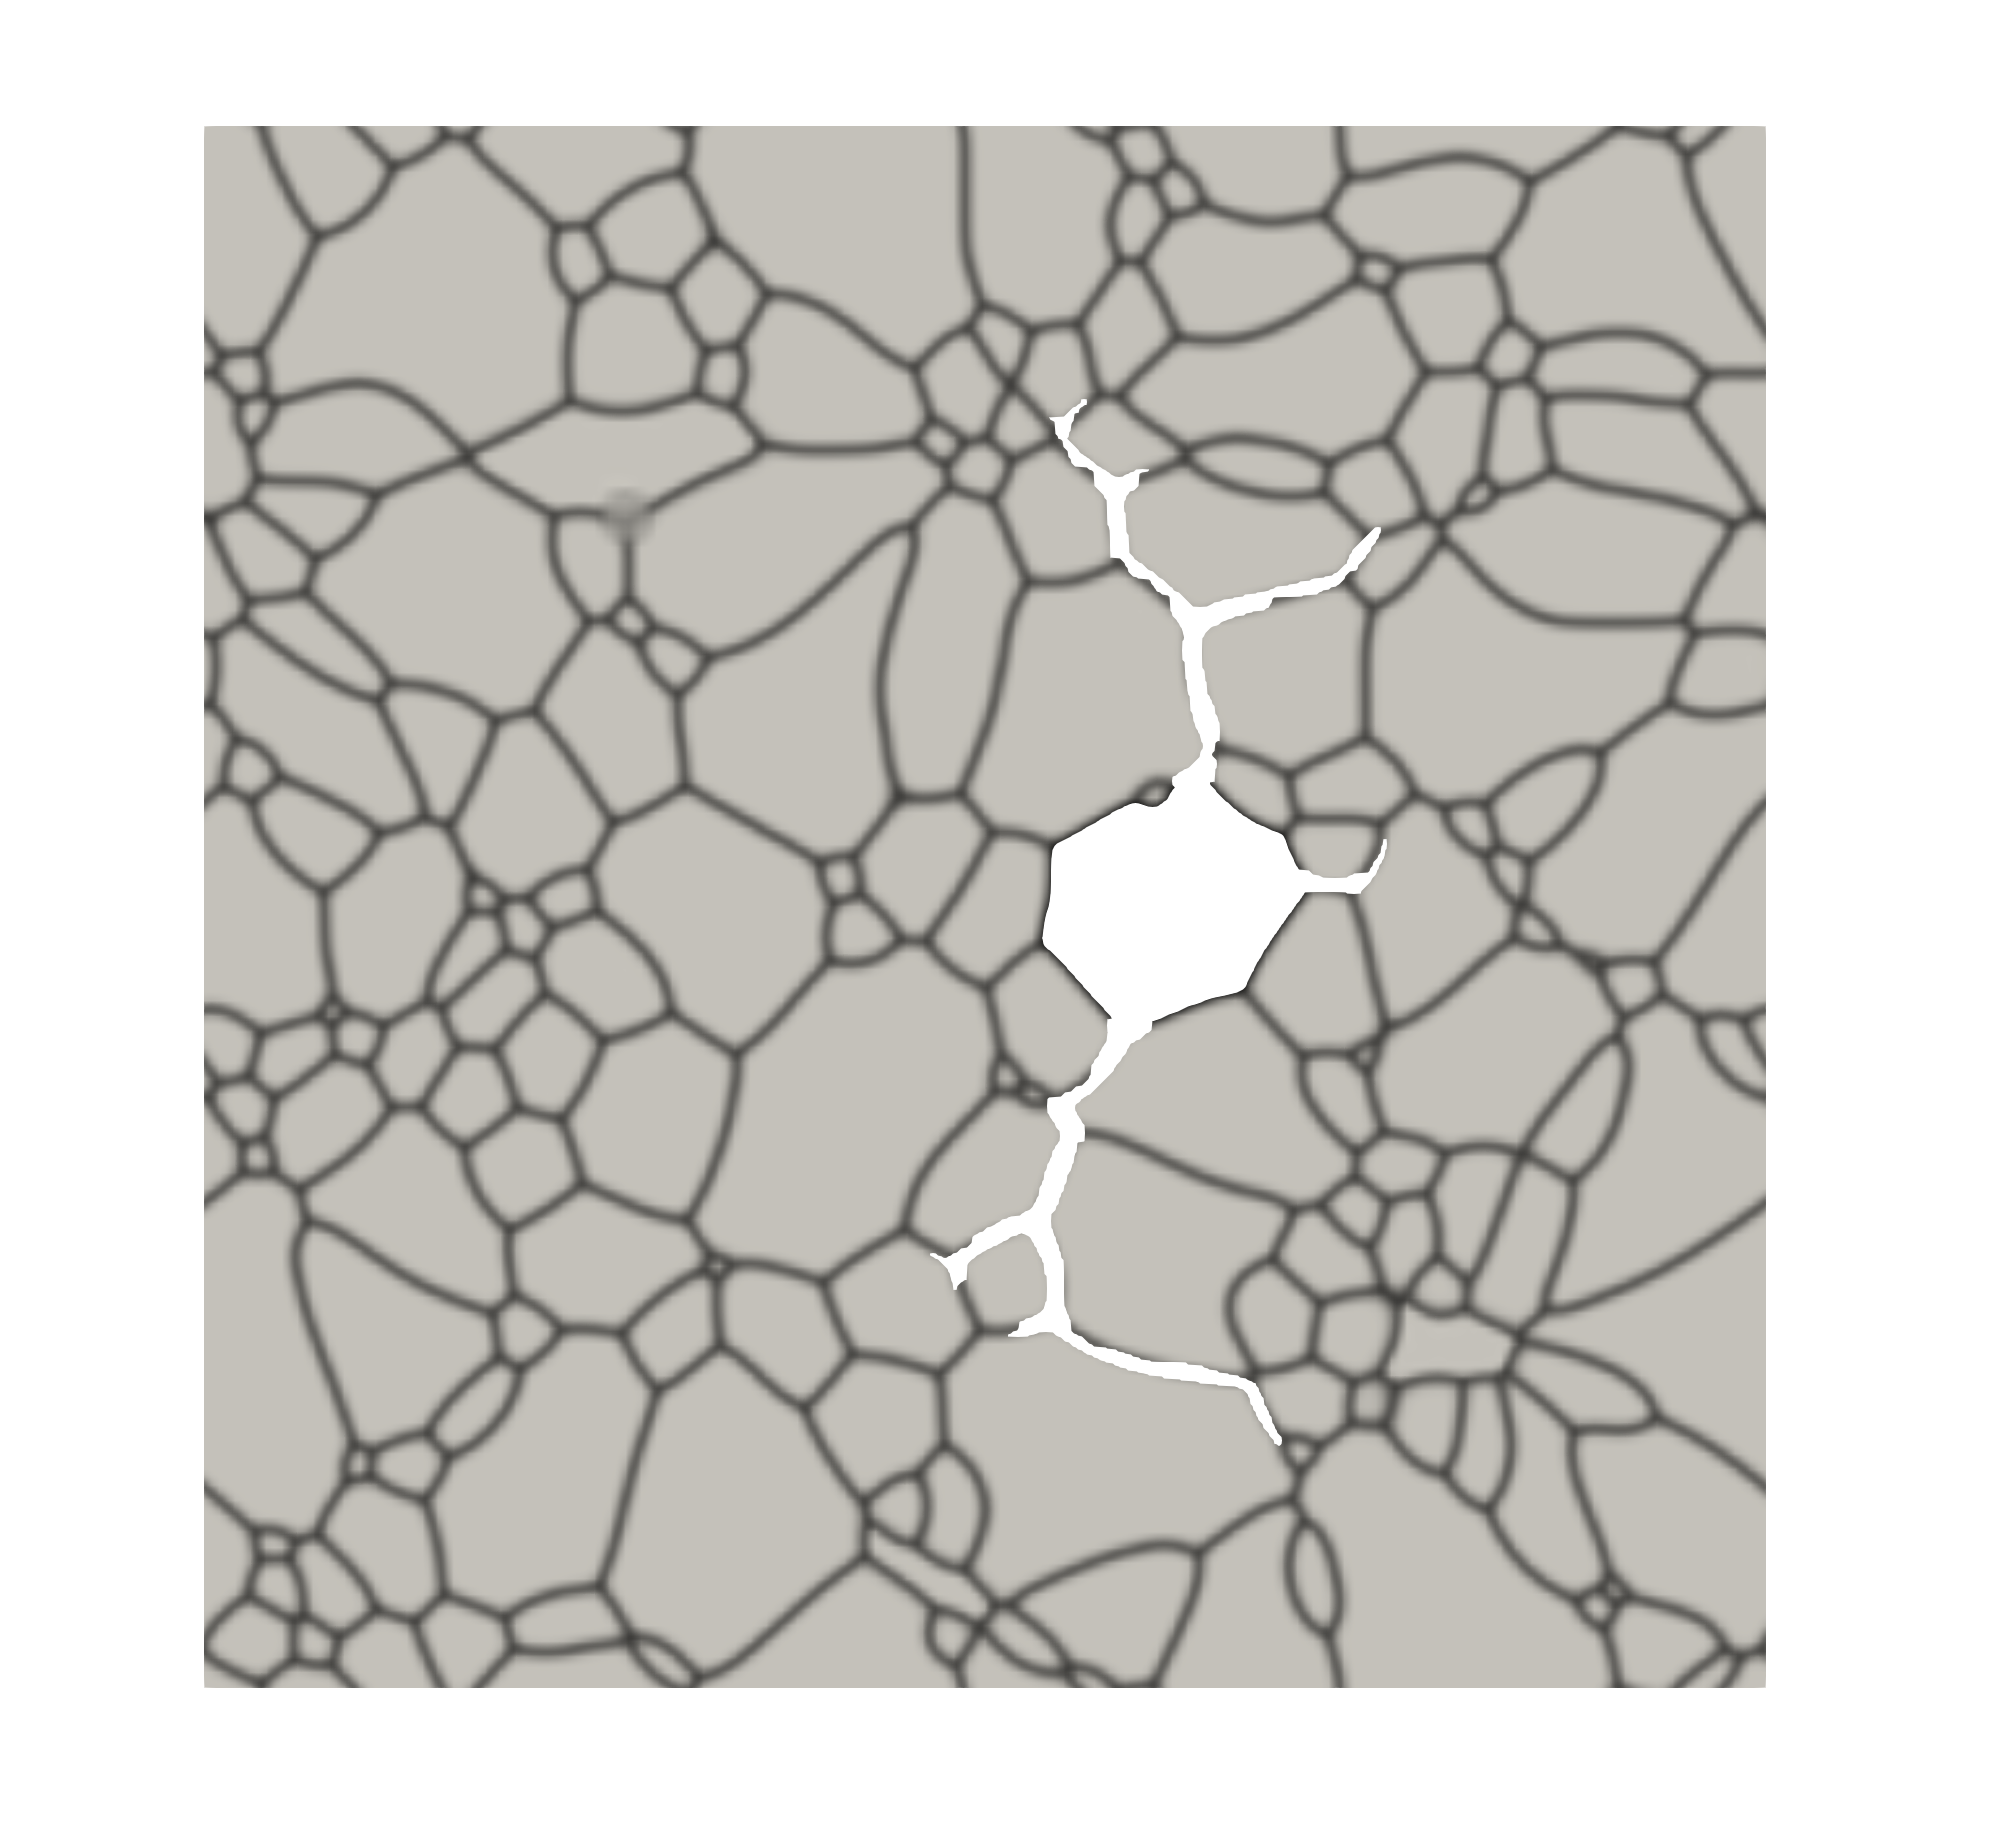
\includegraphics[width=0.9\linewidth]{Chapter345/figures/partial_hbs_3}
        \end{subfigure}
        \begin{subfigure}[t]{0.47\linewidth}
          \centering
          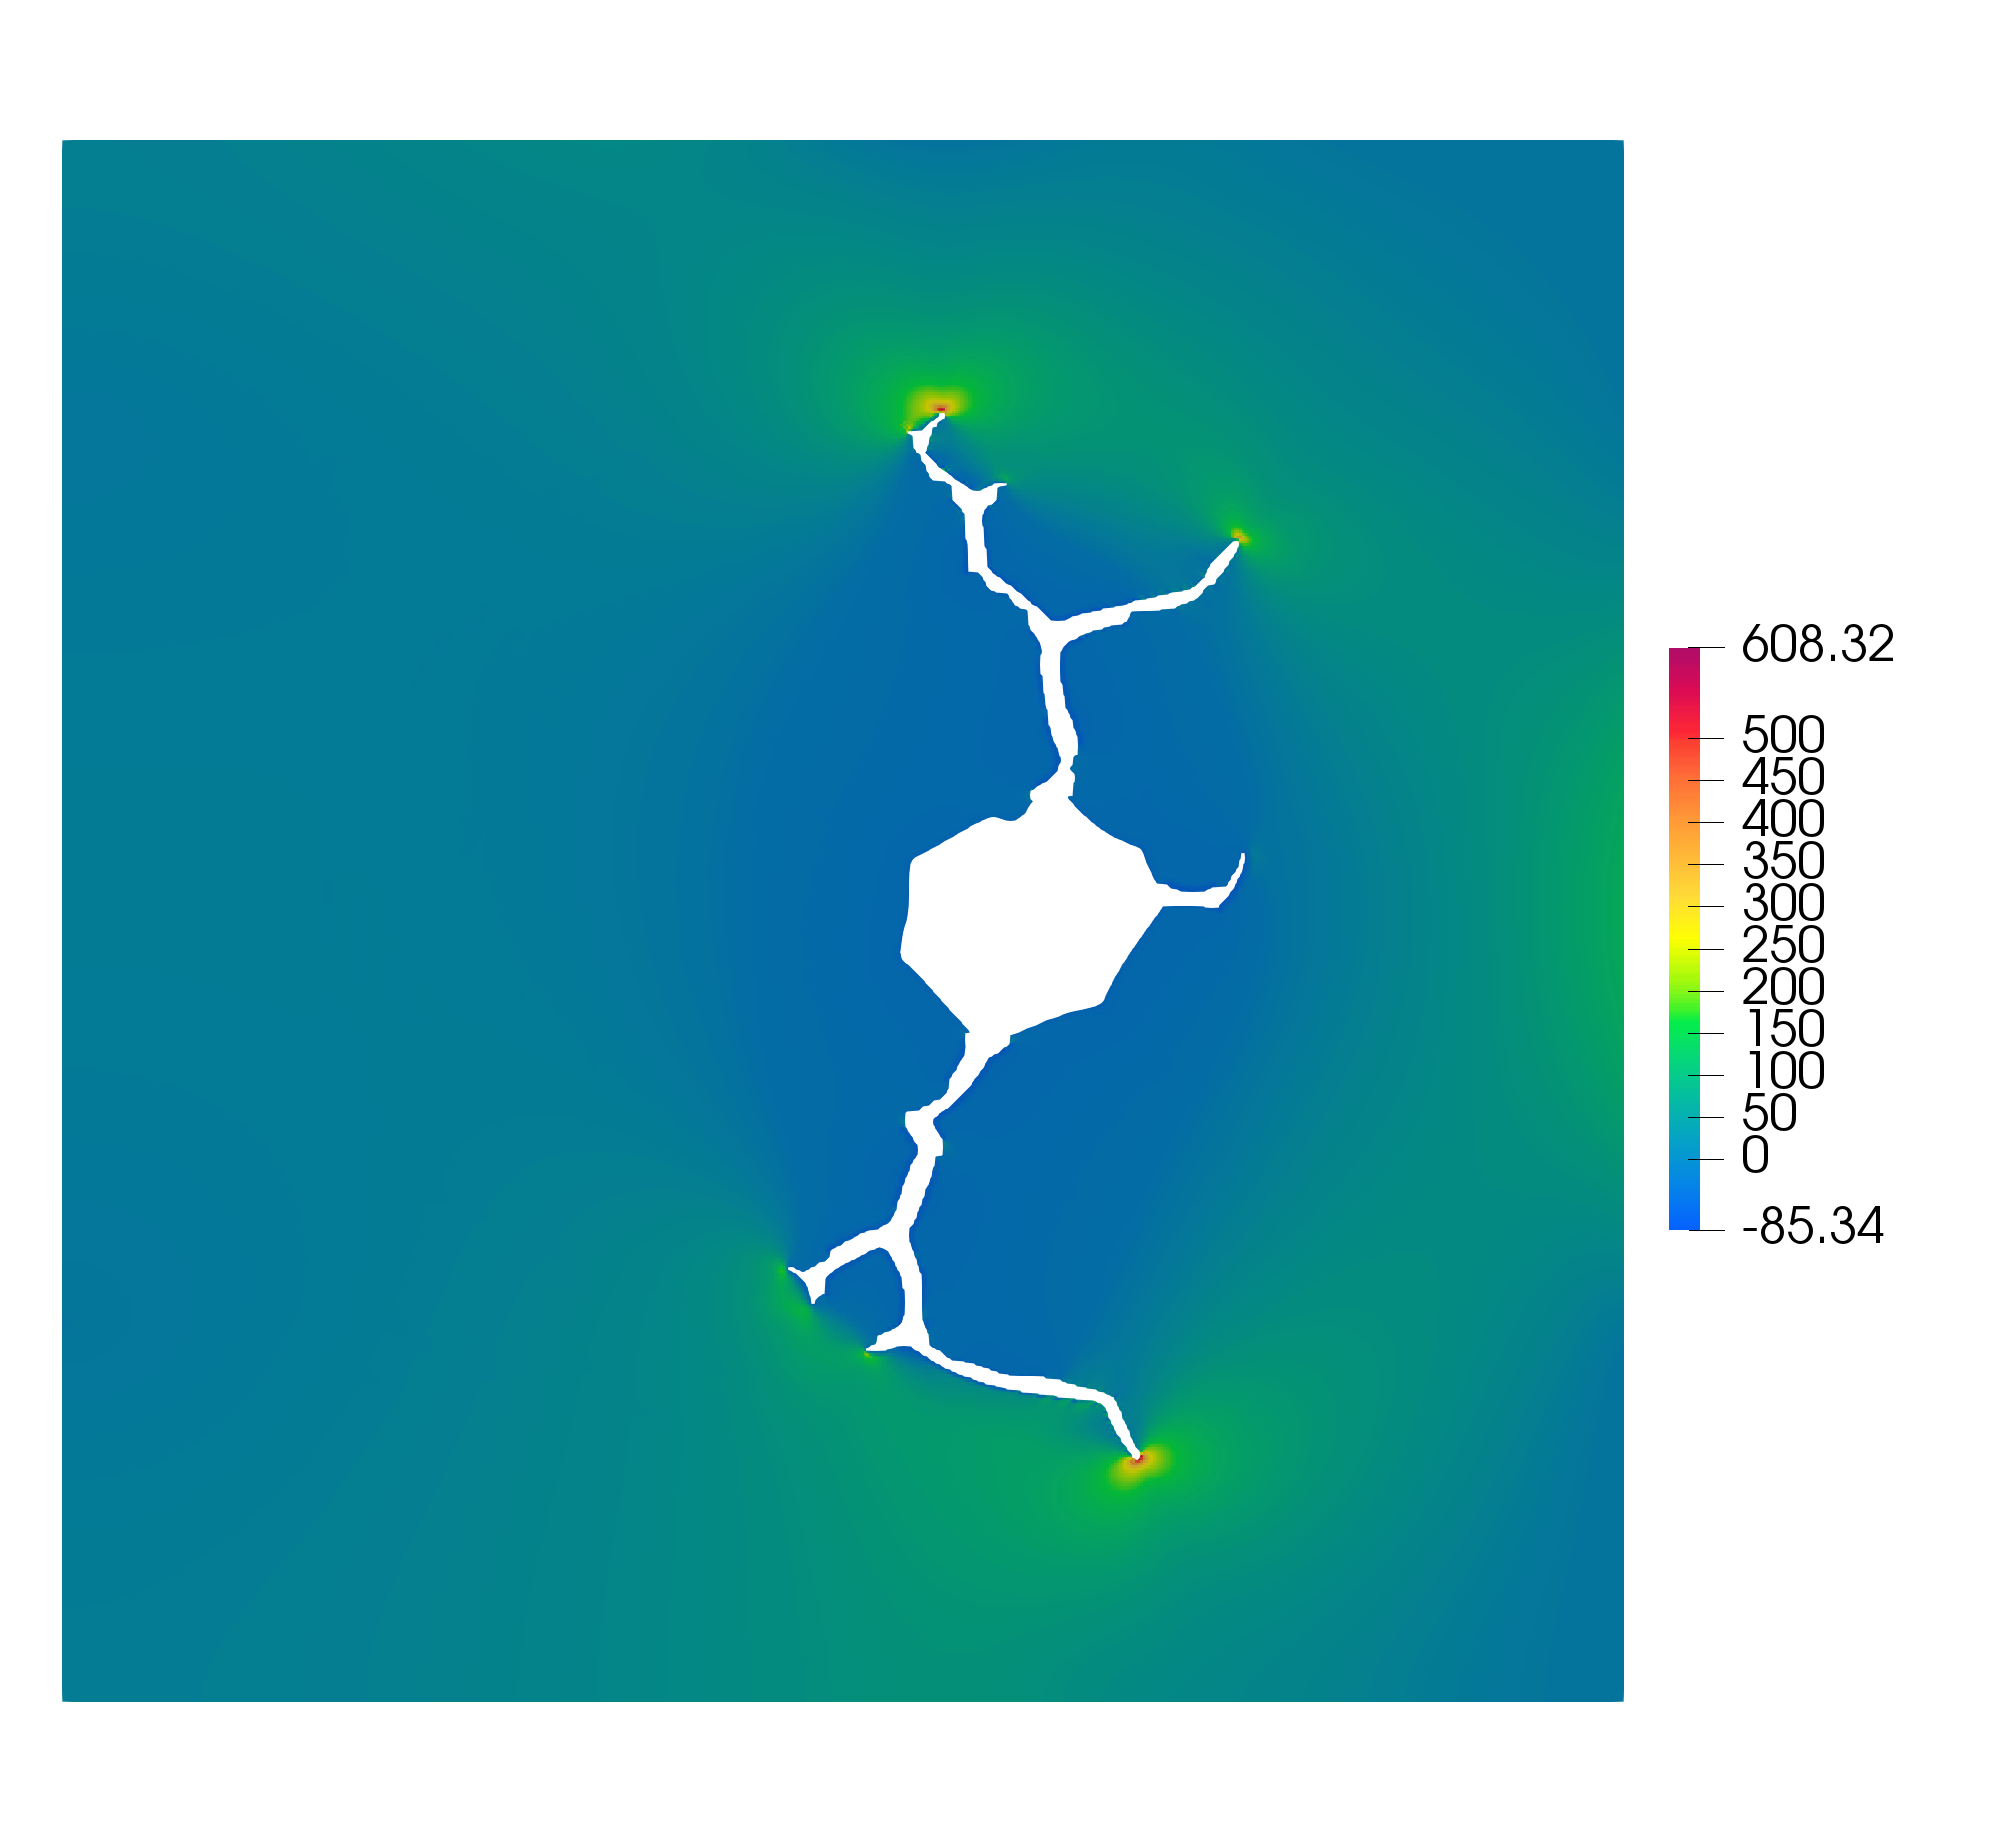
\includegraphics[width=0.9\linewidth]{Chapter345/figures/partial_hbs_3_stress}
        \end{subfigure}
      \end{figure}
    \end{column}
    \begin{column}{0.4\textwidth}
      \begin{itemize}
        \item A 2D REV is considered. Plane strain conditions are assumed to hold.
        \item LOCA pressure transients:
              \begin{itemize}
                \item The temperature as a function of time at the edge of a representative pellet for each rod is obtained from simulations.
                \item The temperature transient is used as an input to a Kim-Kim-Suzuki (KKS) phase-field model \cite{Aagesen2020} to determine the pressure transient.
                \item The pressure transient is treated as a known in the fracture model.
              \end{itemize}
        \item Effects of bubble size, bubble pressure, surrounding pressure, and multi-bubble interaction are investigated.
        \item Defect evolution and recrystallization can be incorporated into the fracture model.
      \end{itemize}
    \end{column}
  \end{columns}
\end{frame}
